%===================================== CHAP 4 =================================

\chapter{Experiments and results}\label{chpt:experiments}

This chapter structures experiments into sub-sections, which also contain a (detailed and somewhat abstract) analysis of the specific experiment results. The research questions and a more general abstract discussion is addressed in the next chapter, \ref{chpt:discussion}.
This chapter begins with a fairly thorough analysis of the hippocampal module. In this analysis several variables are chosen as free variables, for which traditional experiments testing the variables (schemes and configurations) are run. Novel aspects are proposed and implemented according to the attained results, and even further experiments are proposed, performed and analysed.
Roughly speaking, the free variables which are tested in the experiments are initially asynchronous and synchronous updating of the CA3-layer within the hippocampal model, followed by introducing a synaptic connection weighting between the dentate gyrus (DG) and the CA3-layers which is held as a free variable in the experiment. Furthermore, two different neuronal turnover modes, and the neuronal turnover rating itself are instantiated as free variables, resulting in data on different variable values along the aforementioned axes. Lastly, the convergence criterion during learning and recall is reformulated into a slightly less stringent, and more consistent criterion, being training og recalling for a static number of iterations, which results in a basis for further analysis.

Following the analysis on the hippocampal module, is an analysis on memory consolidation to the neocortical network for several of the hippocampal model schemes. I.e. learning by the chaotically recalled and extracted patterns, and by using pseudopatterns.
These address at first properties of the neocortical module itself, being a standard feed-forward back-propagation (FFBP) network. Thereafter, experiments on memory and function consolidation based upon the previously attained chaotic patterns and pseudopatterns, are presented. These form the basis for further experiments and results, and an analysis of the entire dual-network memory model.


\section{Setup}

The initial setup is in accordance with the findings of the literature study, and mainly based on the parametrization used in \citep{Hattori2010, Hattori2014, Wakagi2008}. See tables \ref{table:number_of_neurons}, \ref{table:firing_rates}, and \ref{table:initial_weight_distributions}.

\begin{table}
\centering
\caption{Lists the number of neurons in each layer within the hippocampal module.}
\label{table:number_of_neurons}
\begin{tabular}{l|l|l|l|l|l|}
\cline{2-6}
                              & Input & EC  & DG   & CA3 & Output \\ \hline
\multicolumn{1}{|l|}{Neurons} & 49    & 240 & 1600 & 480 & 49     \\ \hline
\end{tabular}
\end{table}

\begin{table}
\centering
\caption{Displaying the firing rates for the different layers, and the resulting values $k$ for k-Winners-Takes-All.}
\label{table:firing_rates}
\begin{tabular}{l|l|l|l|}
\cline{2-4}
                                  & EC   & DG   & CA3  \\ \hline
\multicolumn{1}{|l|}{Firing rate} & 0.10 & 0.01 & 0.04 \\ \hline
\multicolumn{1}{|l|}{Resulting $k$} & 24 & 16 & 19 \\ \hline
\end{tabular}
\end{table}

% initial weight distribution - Gaussians
\begin{table}[]
\centering
\caption{Displaying the parameters for $\mu$ and $\sigma^2$, with which the weights are normally distributed. Note that the parameters found in the table correspond to the tuple $(\mu, \sigma^2)$.}
\label{table:initial_weight_distributions}
\begin{tabular}{l|l|l|l|}
\cline{2-4}
                          & DG        & CA3       & Out      \\ \hline
\multicolumn{1}{|l|}{EC}  & (0.5, 0.25) & (0.5, 0.25) & n/a      \\ \hline
\multicolumn{1}{|l|}{DG}  & n/a       & (0.9, 0.01) & n/a      \\ \hline
\multicolumn{1}{|l|}{CA3} & n/a       & (0.5, 0.25) & (0.0, 0.5) \\ \hline
\end{tabular}
\end{table}

Furthermore, the DG-weighting is set to either $1$ or $25$, and the neuronal turnover rate to either $0.50$ or $0.04$. The former initial setups being chosen in order to test the configurations of both models on which my implemented model is based, while the latter values are chosen due to the attained success using the first turnover rate, and the second because it is close to the values observed within the biological brain \citep{Rolls1998chpt6}.
The potential impact of increasing the DG-weighting on model performance and pattern separation, as well as varying the neuronal turnover rate under two different turnover schemes, is studied in the experiments (section \ref{section:hpc-experiments}).

\begin{table}
\centering
\caption{Initial model variable constant settings. Neuronal turnover was calibrated through initial experiments along with the CA3 neuronal updating scheme, as well as the DG-weighting.}
\label{table:initial_settings}
\begin{tabular}{|l|l|l|l|l|l|l|l|l|l|}
\cline{1-8}
Parameter: & Gamma & Epsilon & Nu   & k\_m & k\_r & a\_i & alpha \\ \hline
Value:     & 0.70  & 100.0   & 0.10 & 0.10 & 0.95 & 0.80 & 2.00 \\ \hline
\end{tabular}
\end{table}

\subsection{Data set}
As previously mentioned, the input and output layers consist of 49 neurons each. (I MIGHT perform some experiments for 200 I/O with correlated patterns for some config.s later on, in that case: Refactor then). 
% I/O
When it comes to the data that is used, classical experiments of sequentially learning pattern associations, meant to highlight retroactive interference, are adapted. These correspond roughly to the experiments of \citep{McCloskey1989}, as adapted by \citep{French1997, Hattori2010, Hattori2014}.

In this thesis, two sets of 25 distinct patterns are used, namely the first 25 letters of the alphabet, in uppercase for the first set, and in lower case for the second. Each letter is compressed to a 7x7 image of binary pixel values (black or white), corresponding to bipolar input or output values. I.e. bipolar vectors of length 49, where -1 corresponds to black, and 1 to white. Note that the input and output space is significantly reduced by constraining the vectors to bipolar values. (more specifics on this?)

\begin{figure}\label{fig:sample_letters}
    \centering
    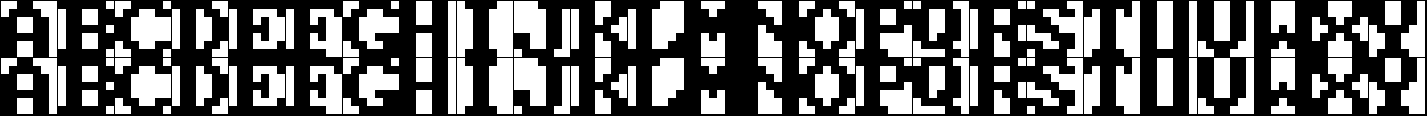
\includegraphics[width=9cm]{fig/im_both.png}
    \caption{Illustrating 7x7 images that are used as input and output patterns, the first row being the input patterns and the second being the associated output pattern, here illustrated for the auto-associative case for the first 2x5 patterns. Note that each pixel value is inflated to a larger square of pixels in order to make the figure more readable.}
\end{figure}


% ========================== EXPERIMENTS ============================          
\section{Hippocampal module experiments}\label{section:hpc-experiments}

Before I introduce the experiments, I would like to briefly introduce the model functionality by demonstrating model activity in a single experiment at a slightly lower and more detailed level. The intention of this is to create a more complete and sound picture of the model elements, as well as to provide the reader with a more thorough understanding of the representations that are used as input and output data. 
This is followed by experiments designed to test specific aspects of the hippocampal model, presenting aggregate results such as graphs of mean convergence ratios along with corresponding analyses.

\subsection{Low-level demonstration}
Following is a demonstration of hippocampal model learning, using two distinct model schemes for two different examples, with figures of model output after each learning iteration for chaotic recall and normal recall, i.e. pattern association. The first two subsets of auto-associative patterns, that is \{A$\rightarrow$A, B$\rightarrow$B\}, and \{C$\rightarrow$C, D$\rightarrow$D\}, are used as training sets in this example.
Furthermore, the hippocampal module is instantiated with the parametrization described above in tables \ref{table:initial_settings} and \ref{table:firing_rates}, and with a neuronal turnover rate $\tau = 0.04$ and a DG-weighting of $1$ in the first example, and $\tau=0.50$ and DG-weighting$=25$ in the second example. Neuronal turnover is performed between every learnt training set - that is, only once after learning the \{A$\rightarrow$A, B$\rightarrow$B\} associations, before commencing learning of the next pair. Here the convergence criteria is set to a static number of training iterations, equal to $15$.
In further experiments, results are generated and analysed for both a dynamic convergence criteria for learning and stability during recall, as well as for two configurations of $i$ training iterations as the learning and stable recall criterion. Furthermore, the weight matrices are instantiated according to their respective firing rates, with weights being randomly assigned according to Gaussian distributions using the parameters presented in table \ref{table:initial_weight_distributions}, for the number of neurons corresponding to the layers' firing rates, respectively (as outlined in table \ref{table:firing_rates}).

Instantiating the hippocampal model using the parametrization as outlined above, images are generated of the network output for pattern recall (i.e. association), and chaotic recall for every training iteration. These are generated for both examples, i.e. synchronous and asynchronous updating of the CA3-layer in the model.

\begin{figure}
    \centering
    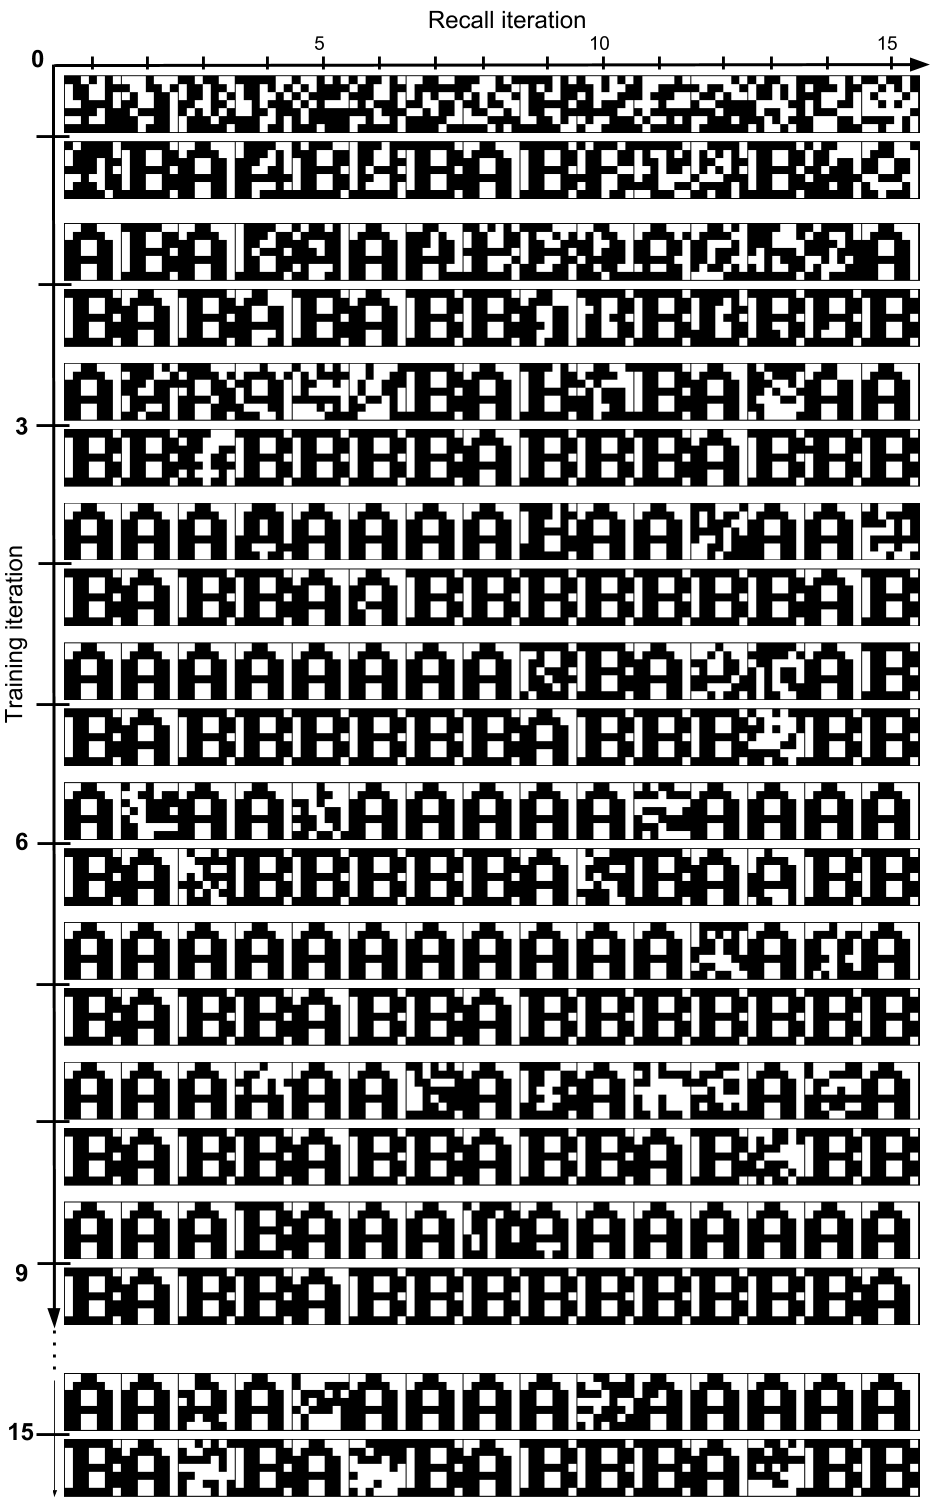
\includegraphics[width=10cm]{fig/AB-pattern-associations-sync-tm0-dgw25}
    \caption{Displaying the recalled pattern for inputs A for the upper row, and B for the lower row, for every learning iteration.}
    \label{fig:pattern_associations_sync}
\end{figure}

\begin{figure}
    \centering
    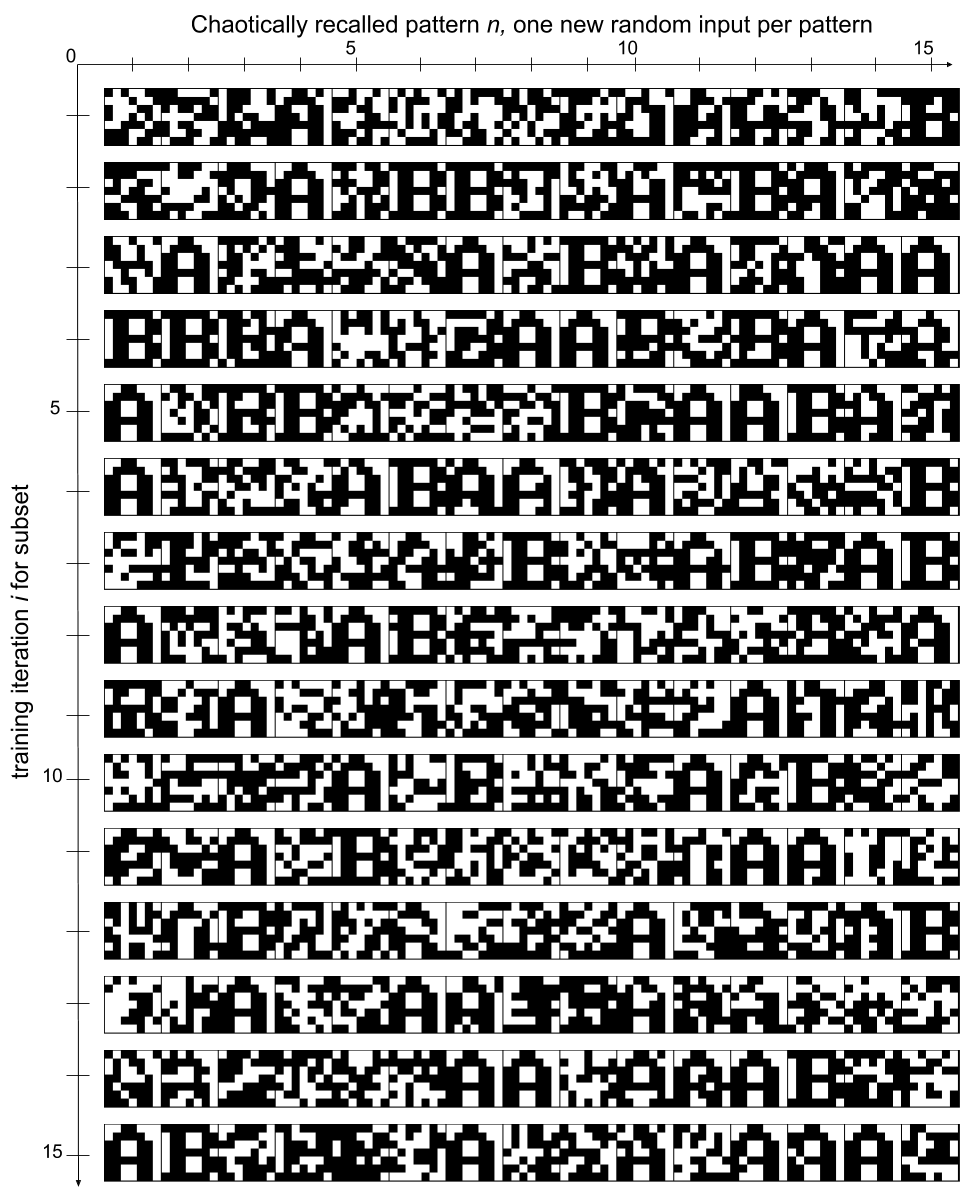
\includegraphics[width=10cm]{fig/AB-chaotic-recall-sync-tm0-dgw25}
    \caption{Displaying the patterns which were recalled by chaotic recall - that is, for each training iteration, 15 patterns were recalled. For each pattern that was recalled, a (new) random input was generated and set as the model's input. Note also that using the same random input also would yield chaotically recalled patterns, which is also included in the trials and experiments contained later in this chapter.}
    \label{fig:chaotic_recall_sync}
\end{figure}

When studying the two figures (\ref{fig:pattern_associations_sync}, \ref{fig:chaotic_recall_sync}) that display the recalled patterns during and after learning pattern-associations for patterns A$\rightarrow$A, and B$\rightarrow$B, note that pattern separation seems fairly successful, as the associated output for the aforementioned letters is fairly stable. However, some spurious patterns appear, even in the case of having the actual, non-distorted input of the pattern as the model's input. This may indicate only a weak model convergence, which may be due to incorrect model calibration, such as too heavy a DG-weighting. Because the connections from the DG-layer are both instantiated normally distributed with rather high values ($\mu=0.9, \sigma=0.01$), and weighted 25 times stronger than the connections from the EC- and CA3-layer, this may possibly disrupt the strength of the attained basins of attraction, or prolong the training period needed in order for the model to converge for its (EC-CA3, CA3-CA3, and thus CA3-output) connections, and thus for the CA3-layer to extract non-overlapping pattern-associations. The latter resulting in instable behaviour within the auto-associative CA3-layer. Now, one run is not sufficient to determine whether this is the case. Therefore, these are parameters that will be tested in further experiments, where 20, or at least 10 trials per training set size, per configuration, are used in order to statistically determine patterns of the emergent model behaviour. I.e. At least 40-80 experiments per model configuration.
Lastly, it is worth noting that although model convergence and recall is fairly good in the case of having a non-distorted training pattern input as input, a great number of spurious patterns are recalled in the chaotic recall scheme. Thus, the number spurious patterns extracted from chaotic recall is one of the measures that will be used in further analyses. Particularly with regards to successful pattern separation and the establishing of basins of attraction. I.e. the perfect recall rate may be erroneously observed as close to 100 \% of the number of training patterns - however, when the number of spurious patterns extracted by chaotic recall exceeds this number (possibly by a great deal), the quality of the model performance may still be considered poor. Note, however, that it might be interesting to also consider memory consolidation in such a scheme to the neocortical module. I.e. whether a functional mapping is yet contained in the spuriously recalled patterns - as given random inputs may still determine a functional mapping to a seemingly spurious output. Note that in the case of attaining a spurious pattern output for an input from the training set, the functional mapping is most likely not present, and will only disrupt the convergence in the network which attempts to learn the pattern-associations. When it comes to the measures of model performance, another measure which will be used in terms of pattern consolidation is the goodness of fit measure, defined in the previous chapter (\ref{chpt:methods}).

% Furthermore, this instability, or oscillation between the model's basins of attraction, is further demonstrated in the figure of chaotically recalled patterns, which barely recalls the letters A and B, and mostly only spurious patterns that do not resemble the original input nor output patterns. Pattern separation is one of the aspects that are evaluated in this thesis. It is evaluated through successful convergence in the first configurations where the convergence criteria is defined as the output being stable for three iterations of recall. Furthermore, it is analysed in terms of all the configurations by considering the perfect recall rates, as well as spurious pattern recall rates.

In order to demonstrate another hippocampal model configuration, low level results are presented below for the case of asynchronous updating of the CA3-layer. Neuronal turnover is still only performed between the two learning sets, which may be argued to be biologically unrealistic (some recoding of weights, i.e. topological synaptic modification) may be argued to be continuously present, at a low rate. The latter is something that will be addressed in later experiments. Nonetheless, this constructed low level example introduces randomness in its training and recall by non-synchronously updating the neurons of its CA3-layer for each training and recall iteration. This may be considered to be somewhat more biologically realistic, although still implausible in terms of only one neuron is updated at a time (algorithmically). In a more biologically realistic model, all neurons should be updated simultaneously, where hard-ware level parallelism could potentially determine a pseudo-random order of neuronal updates, making sub-sets of neurons fire and wire simultaneously. 
However, as aggregate activity on the population level is what is studied in this thesis, I consider the attained results to yield valid data, including associated suggestions at the neural network level.

\begin{figure}
    \centering
    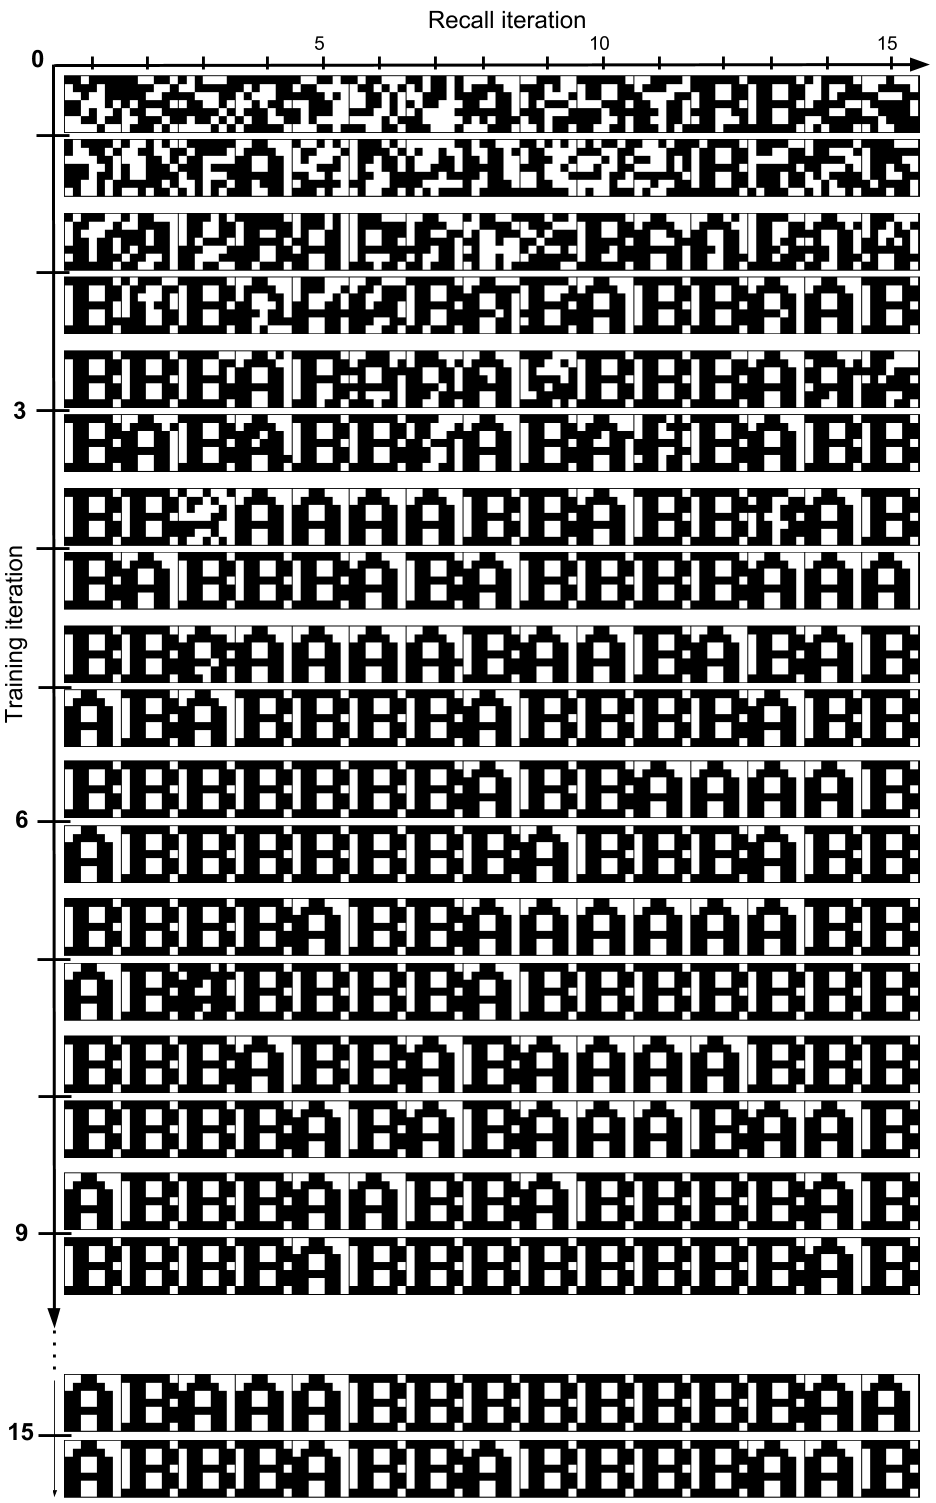
\includegraphics[width=10cm]{fig/AB-pattern-associations-async-tm0-dgw1-tau050}
    \caption{Showing the recalled images after each recall iteration for 15 iterations, for every training iteration of the 15 training iterations. Note that there are two sets of recalled images for each training iteration. The first correspond to recall for input 'A', and the latter for input 'B'. Furthermore, the model configuration used here is asynchronous CA3 udpating, neuronal turnover between every learnt set, a DG-weighting of 1, and $\tau=0.50$.}
    \label{fig:low-level-3}
\end{figure}

\begin{figure}
    \centering
    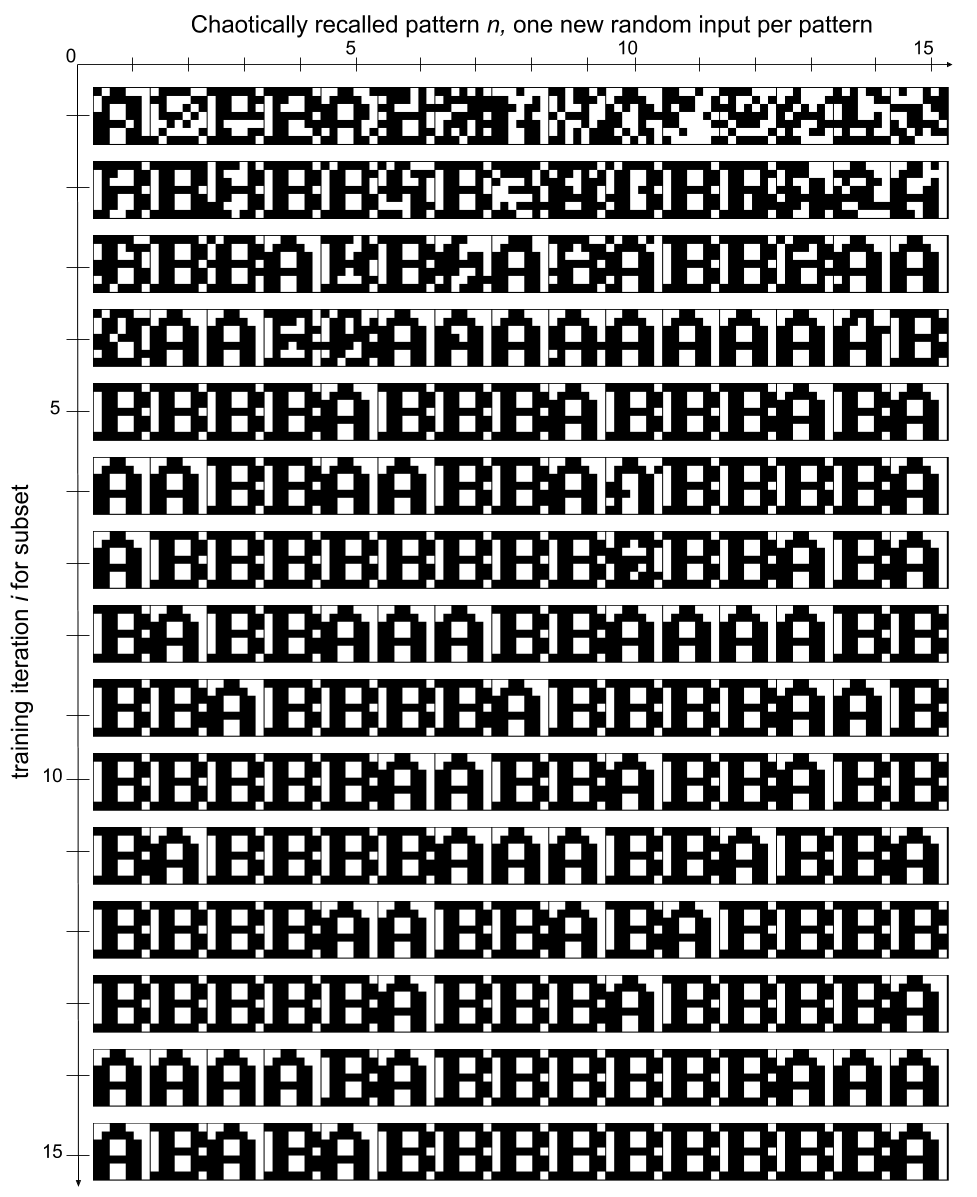
\includegraphics[width=10cm]{fig/AB-chaotic-recall-async-tm0-dgw1-tau050}
    \caption{Displaying the chaotically recalled patterns for the same model configuration and results as displayed in figure \ref{fig:low-level-3}. Note that spurious patterns diminishes very quickly, and only learnt patterns are chaotically recalled after very few iterations. This configuration seems to be capable of one-shot learning.}
    \label{fig:low-level-4}
\end{figure}

Note that while the quality of chaotic recall appears to be better in figures \ref{fig:low-level-3}, and \ref{fig:low-level-4}, the scheme is less stable for the output for a learnt pattern association's input. This is expected, as more randomness is introduced in the random sequence of updating the neurons of the CA3-layer, which will tend to have the model find the other basin of attraction more easily. Because these results were attained only from one run, the generalisability is somewhat constrained. Nevertheless, the results do suggest a trend towards a more specific extraction capability at the cost of less stability. It is worth keeping this in mind when considering further experiment results. If the reader wishes to see the figures presenting the attained output for the next training set, i.e. subset of the training patterns, please refer to appendix E, in which they are contained.


\subsection{Experiment 1: Schemes for updating the CA3-layer and performing neuronal turnover}

In order to evaluate the impact of synchronous action potential propagation and synaptic weight modification, four different model schemes are used. These consist of combining two types of CA3-layer neuronal activation and weight modification with two types of neuronal turnover. More specifically; updating the CA3 neuronal activation values synchronously or asynchronously, and performing neuronal turnover between every learned training subset, or for every training iteration. Synchronous CA3-layer updating effectively results in reducing the propagation of values from one layer of neurons to another to a set of vector and matrix operations, whereas the asynchronous scheme requires updating each neuron independently. In the simplest case of synchronous updating, i.e. for all non-chaotic layers, the synchronous propagation scheme is simply reduced to a vector of activation values multiplied by a weight matrix, which is adjusted through the activation function. For each of these schemes; synchronous or asynchronous updating, two turnover modes are tested. Firstly, turnover is performed only once before every new training subset, i.e. between learnt training sets. Secondly, turnover is performed between every training set iteration, i.e. for every iteration over the current subset.

In this experiment, 20 trials is performed for every full auto-associative training set (that is 2x5, 3x5, 4x5, and 5x5), for every configuration. In other words, for 20 trials $20 * 4 = 80$ experiments are run for each model configuration. In these experiments the model attempts to learn to associate the for $n$ first capital letters auto-associatively, where $n$ corresponds to e.g. $2x5 = 10$, $3x5=15$, $4x5=20$, or $5x5=25$, the x denoting that the training set consists of 5 subsets that are used to train the model, sequentially. 
Furthermore, the convergence criterion is defined as the following: For each training pattern in the current training set, if the model output is the correct pattern output for the undistorted pattern-input for three recall iterations, the pattern is considered to be successfully learnt. If this is the case for every pattern in the current training subset, convergence is considered to be attained, and chaotic recall is performed. Furthermore, when generating figures, the model is considered to have successfully learned the current training set if converging in less than 50 training iterations. Chaotic recall is performed similarly to the procedure in \citep{Hattori2010, Hattori2014}. That is, during chaotic recall, when the output remains unchanged for three recall iterations, the pattern is considered to be learnt, or successfully extracted in the case of chaotic recall. Chaotic recall is always performed for 300 time-steps, with the input to the network being a new non-changing random input for every extracted pattern.

% \begin{figure}
%     \centering
%     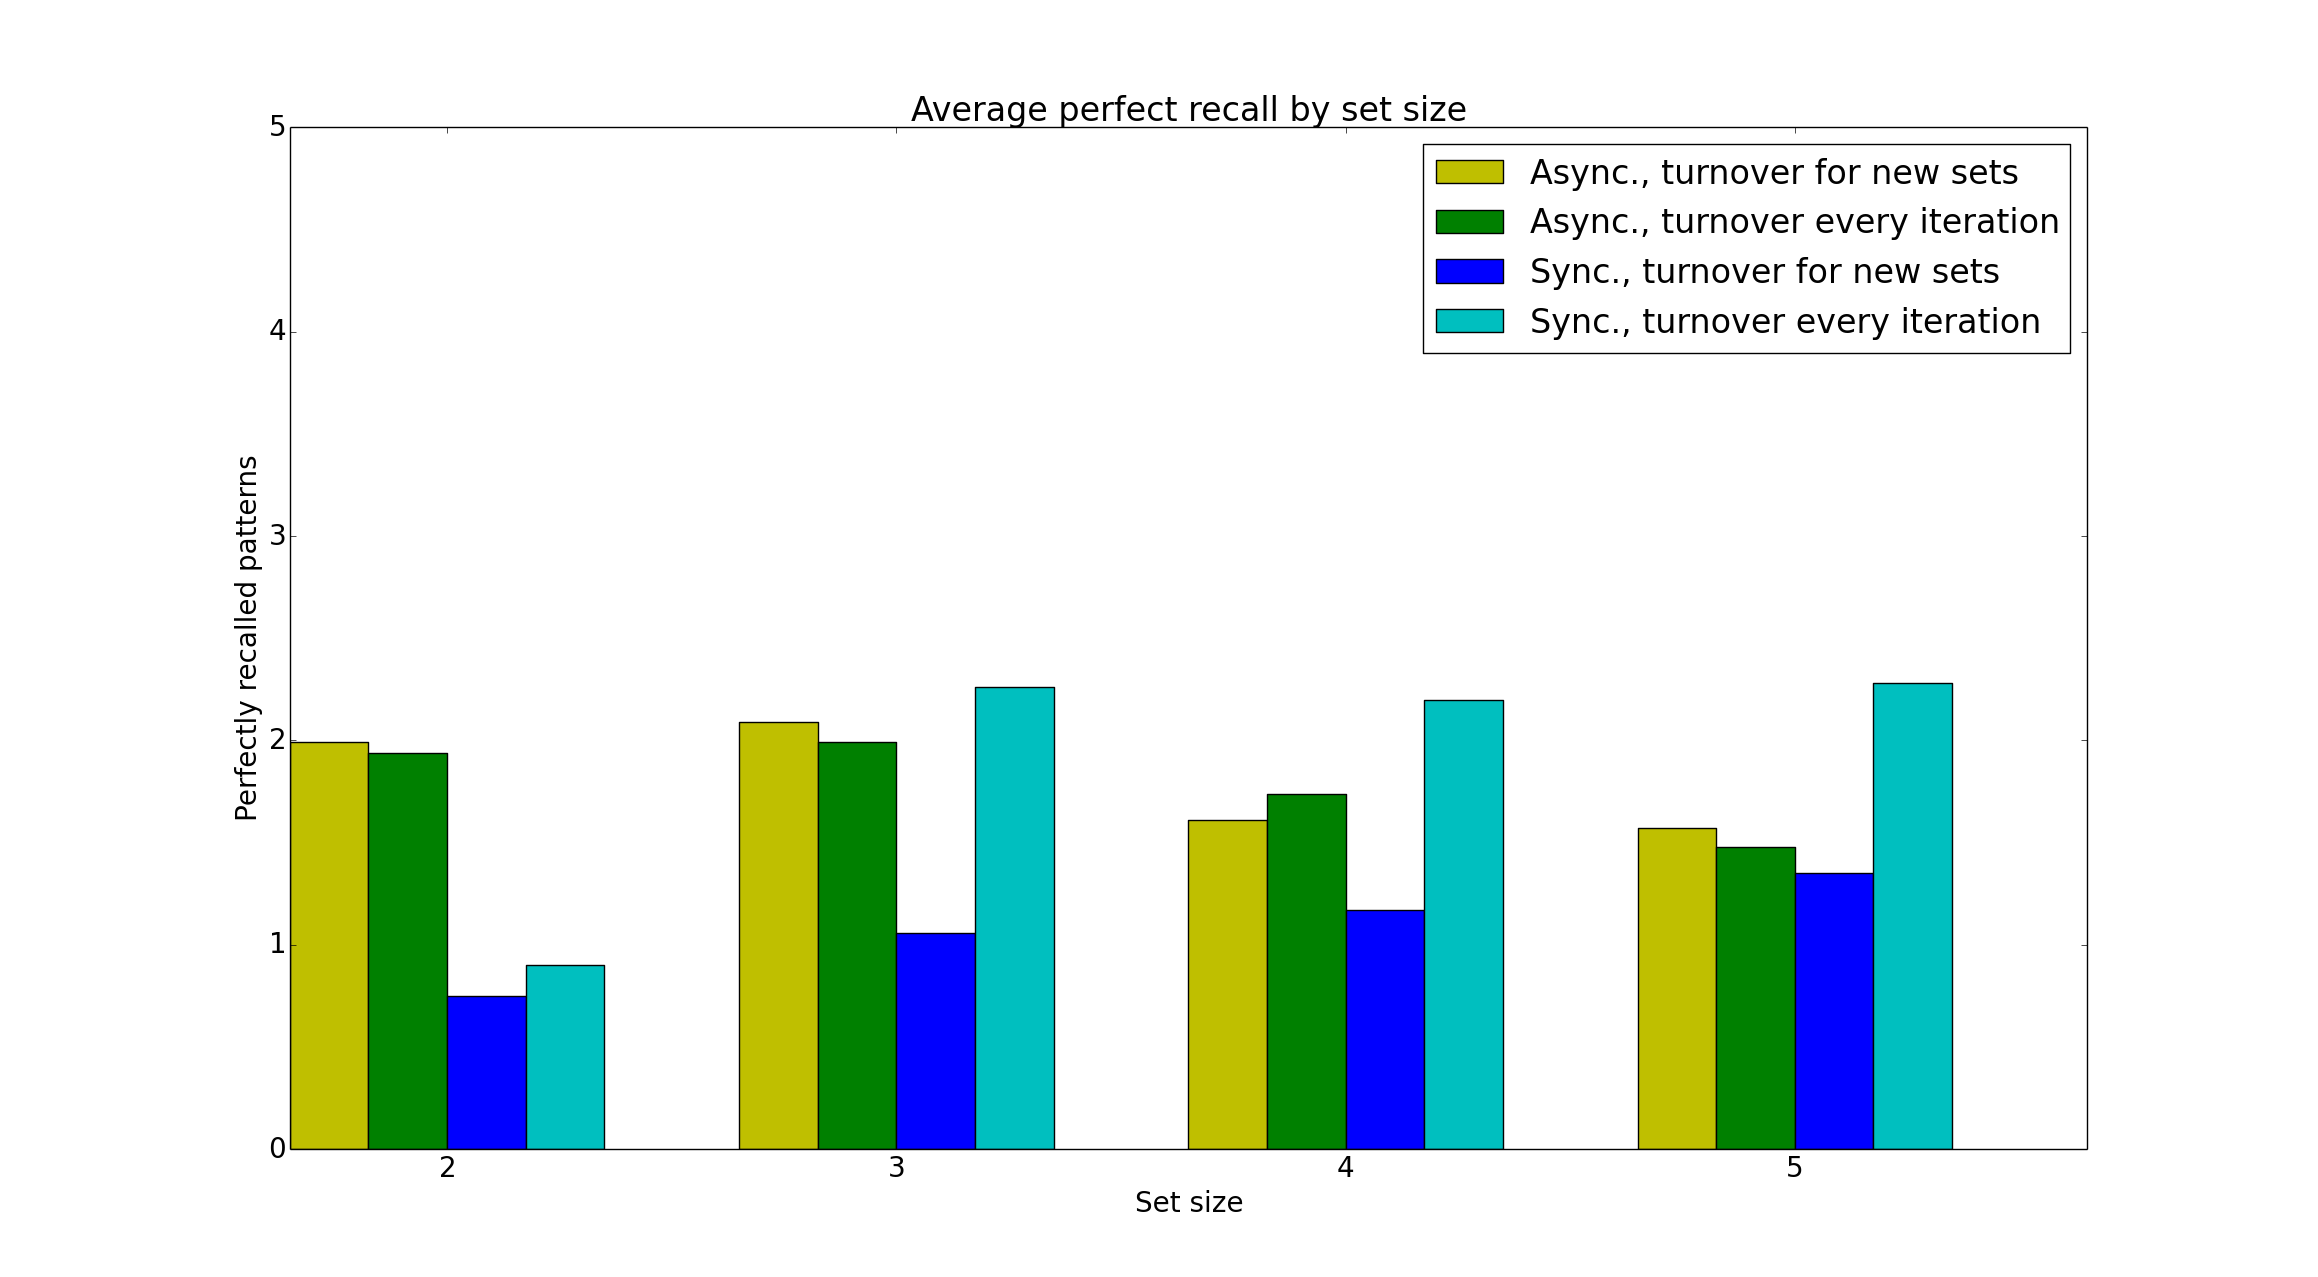
\includegraphics[width=14cm]{fig/average_perfect_recall_rates_by_set_size_bars_reset_for_every_experiment}
%     \caption{Displaying the average number of perfectly recalled patterns by set size for the four different model configurations. Note that the dentate gyrus weighting is set to 25, and the turnover rate to $0.50$ in all of the configurations, which might impact particularly the turnover mode in which turnover is performed between every training iteration.}
%     \label{fig:avg_perfect_recall_bars}
% \end{figure}

\begin{figure}
    \centering
    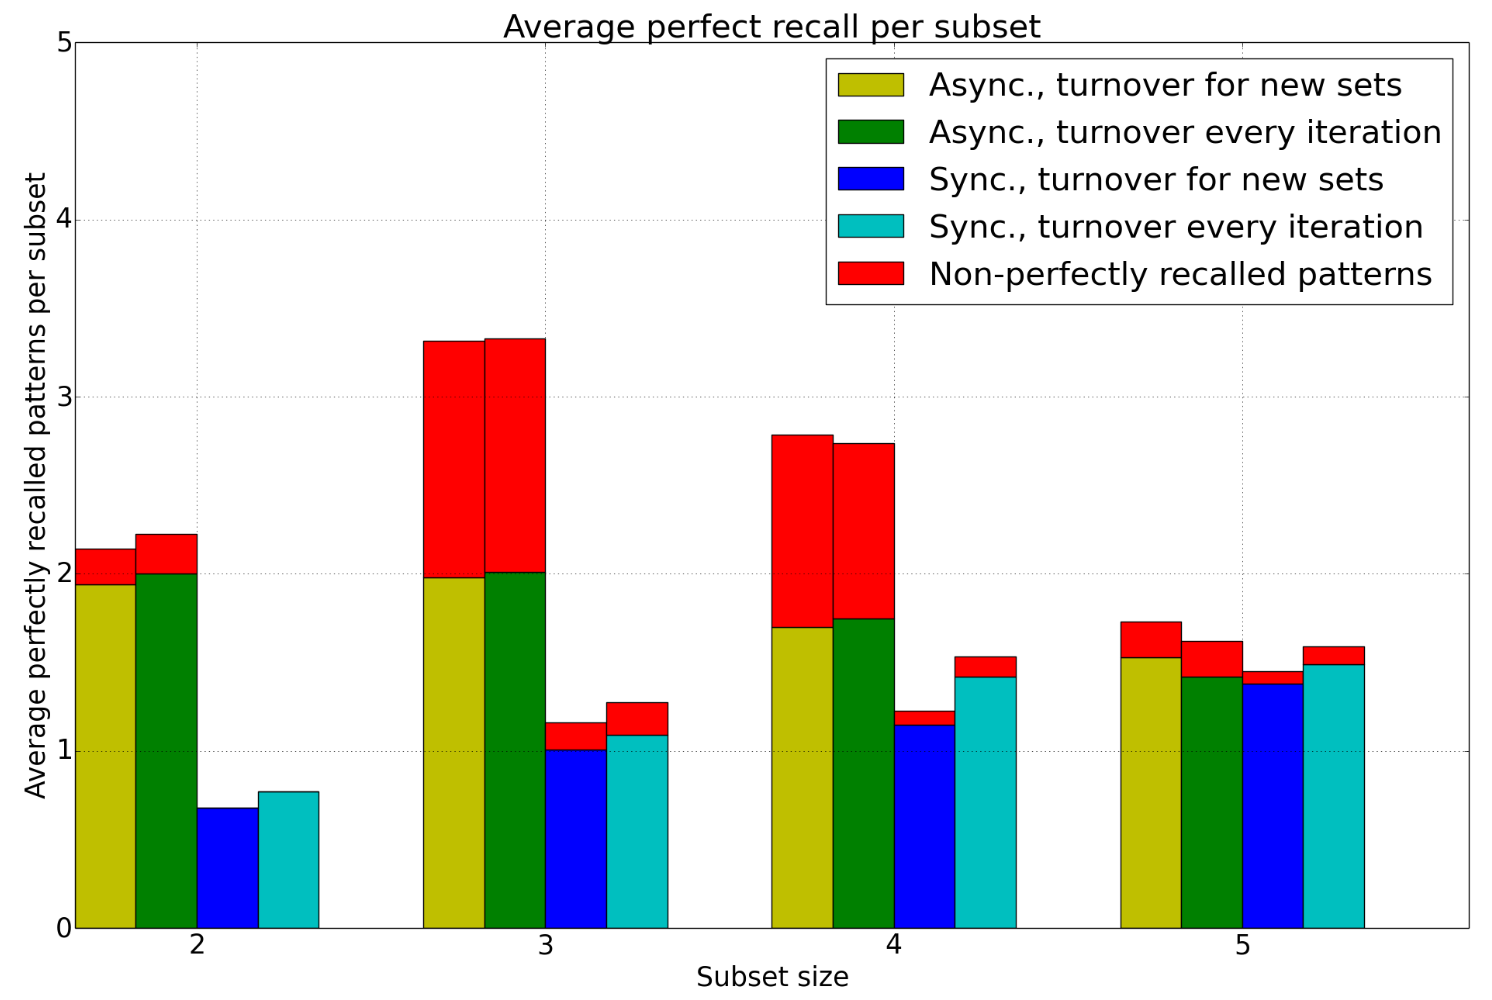
\includegraphics[width=12cm]{fig/average_perfect_recall_rates_by_set_size_with_spurious_bars_cut}
    \caption{Displaying the average number of perfectly recalled patterns for each mode configuration, along with the average number of spuriously recalled patterns for each configuration. Note that the dentate gyrus weighting is set to 25, and the turnover rate to $0.50$ in all of the configurations, which might impact particularly the turnover mode in which turnover is performed between every training iteration.}
    \label{fig:avg_perfect_recall_rates_with_spurious_bars}
\end{figure}

Note that spurious is defined as any distinct non-perfectly recalled pattern in figure \ref{fig:avg_perfect_recall_rates_with_spurious_bars}. Non-perfect is used as a term rather than imperfect to signify that the pattern may be either nearly perfect, or in fact completely random, i.e. spurious. Note that in contrast to the introductory examples where the convergence criterion was defined as training or recalling for a fixed number of iterations \textit{i}, (\textit{i} $=15$ in the introductory low-level examples), having a stricter convergence criterion naturally resulted in no spurious patterns being recalled in the synchronous updating schemes, as may be expected when considering figure \ref{fig:chaotic_recall_sync}. However, it remains unclear whether model convergence is attained only by studying this figure. In order to possibly elucidate this, the convergence rate is also logged and presented in figure \ref{fig:convergence_rates_async_sync} for asynchronous CA3 updating.

\begin{figure}
    \centering
    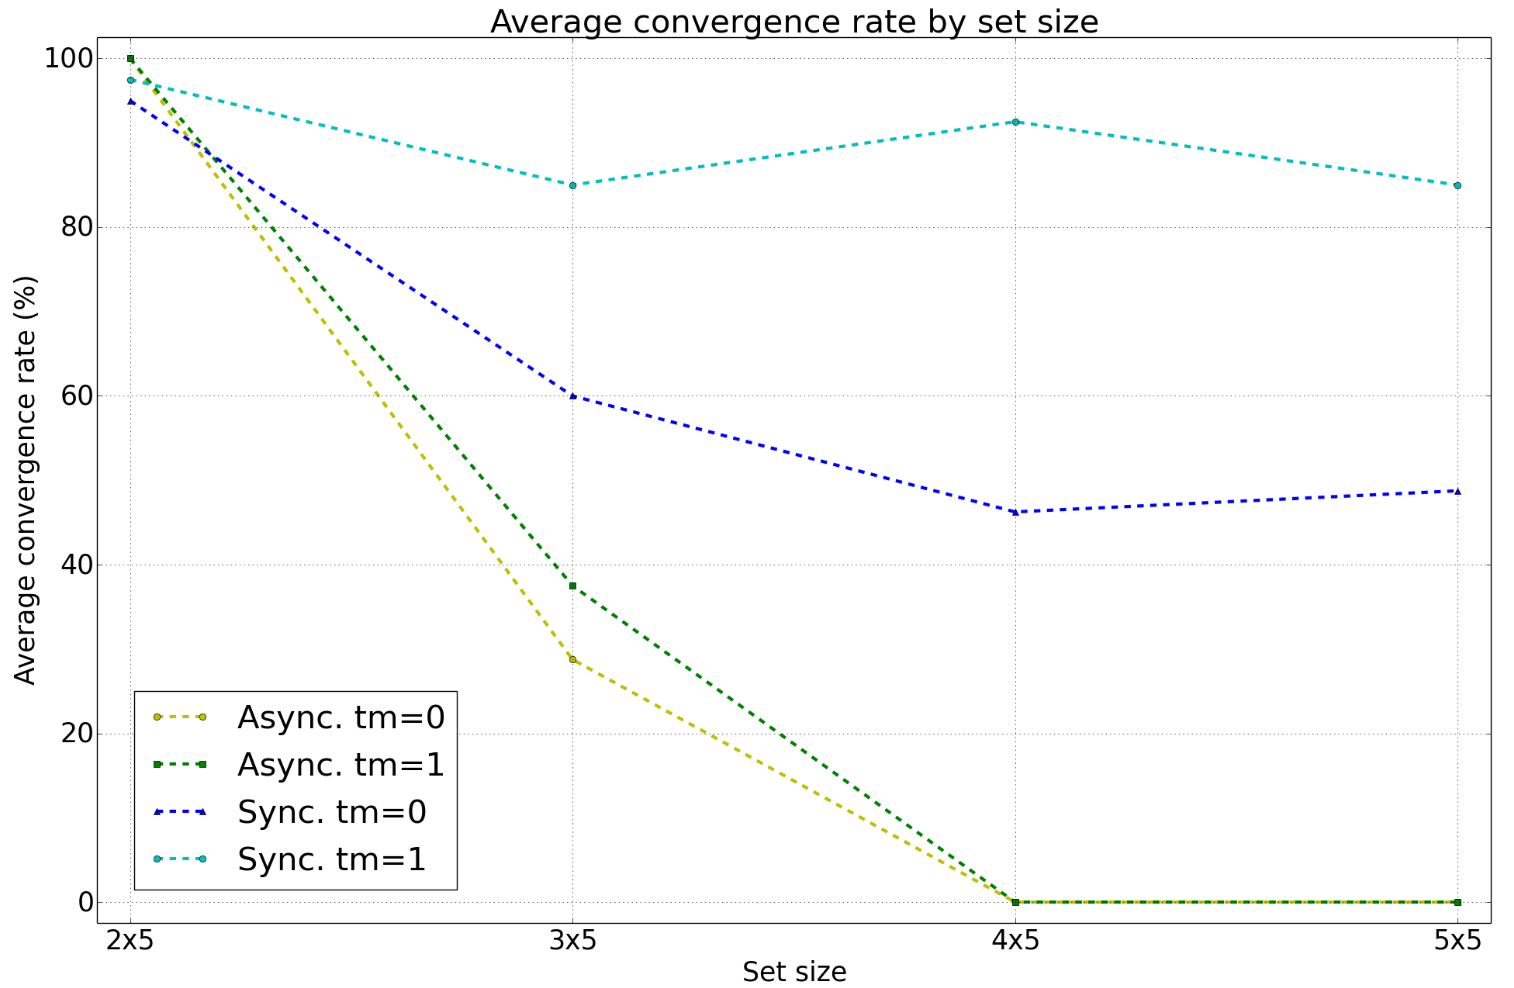
\includegraphics[width=13cm]{fig/avg_convergence_rate_cut}
    \caption{Presenting the average convergence rate in the four experiment-schemes, using the strict convergence criterion. Learning and convergence is considered successful if attained within 50 training iterations. Note that the synchronous updating schemes seem to converge just as well in nearly all cases, except for in the case of set size 5.}
    \label{fig:convergence_rates_async_sync}
\end{figure}

Although extraction of all patterns using chaotic recall is unsuccessful in nearly all of the current experiment schemes, the synchronous schemes converge well for all set sizes, apart from when using turnover for every set iteration for the largest set size (5x5). It is worth emphasizing that the scheme with the best convergence rate converges for nearly 100 \% of the training subsets for all set sizes. However, it remains the scheme which performs the worst in terms of perfect recall, the scheme being synchronous CA3-layer neuronal updating performing neuronal turnover only between learnt subsets. 
Furthermore, this scheme recalls nearly no other than 1-2 of the patterns from each training subset, which it recalls perfectly. This may suggest that while the scheme is likely to successfully be able to separate patterns during training, it does not separate them well enough to be able to chaotically recall them.
Some hypotheses on why training is successful in nearly all cases, but not extraction by chaotic recall, include the following:
- It may simply be that the model adjusts its weights too heavily towards the present firing patterns. However, this hypothesis remains implausible as the convergence criterion ensures that the model is fairly stable for every pattern in the training subset, i.e. the output remains correct for three recall iterations when the corresponding input of the pattern is presented to the network. This is the case in nearly 100 \% of the training cases, unaffected by set size.
- Because every neuron of the CA3-layer is updated synchronously, the model lacks 'jiggle' during recall, making it prone to being stuck in a subset of its basins of attraction. This view is further strengthened by considering that the DG-layer is not used during recall, as it performs expansion encoding, which along with its sparsity may recode and separate similar, but distinct, inputs into separate patterns for the CA3-layer to then be able to auto-associatively learn. Because convergence is attained during training, but not recall, this suggests that the DG-layer may in fact give rise to these emergent qualities, but that the CA3-layer possibly favours a subset of the learnt patterns too strongly, resulting in pattern completion for only this subset of patterns.
- Another view, which of course may very possibly be intertwined with the former is that
Note that due to the quick convergence qualities of the hippocampal module, it is unlikely that the EC to CA3 connections, as well as the CA3-CA3 connections have not been able to converge towards the solution. However, if the recoding does not settle into a steady pattern, changing the input to the CA3-layer significantly for every training iteration, it may of course be the case that the weights do not converge. This theoretical scenario, however, is even more unlikely to occur, as k-WTA will strengthen the connection weights to the first k winners, thus tending to favor the initial winners for the same input, only changing the output which it projects to the CA3-layer very little, if at all. 
This is exactly the reason for why neuronal turnover is performed in the first case - to recode the weight configuration such that the resulting k winners will vary slightly more, thus furthering its recoding abilities, potentially improving pattern separation and model performance. Note that it is the expansion encoding and sparsity in the DG-layer that recodes and separate similar, but distinct patterns. Together with the input of the EC-layer, the current values of the CA3-layer results in updating of weights for the recurrent connection to the layer itself, as well as backwards through the DG- and EC-layer, which again are adjusted according to the 'observed' input for the current pattern. In other words, we seek a configuration for which the model dynamically separates patterns due to its recoding qualities, and yet is able to recall them without the use of the pathways which expand, recode and project its values which separates the patterns. It may be argued that completely omitting this layer during recall is somewhat unrealistic. 
% refactor:
However, according to physiological findings, this pathway is used very little during recall \citep{Wakagi2008}. 
Furthermore, due to the auto-associative nature of the CA3-layer, if this layer has successfully converged for patterns with little overlap, it is likely to fall into a basin of attraction, performing pattern completion for partial pattern input. Now, one may think that the EC-layer will not necessarily project a partial, recoded pattern to the CA3-layer, as this recoding is performed in synergy with the DG-layer. However, as the observant reader may have noticed, it is exactly that; in \textit{synergy} with the DG-layer. As recoding has already been performed, this recoding is propagated to all layers of the network model by Hebbian learning. In other words, the synaptic weight modification between the EC-layer and CA3 will reflect the recoded pattern.
Lastly, the nature of the CA3-neurons, i.e. chaotic neurons, may also impact the chaotic recall capabilities of the model. While it appears evident that the zeta- and eta-equations do not limit successful training of patterns, it may be that they impact the next activation values of the CA3-layer too heavily during recall. This may be argued by considering that in the current implementation, the next eta- and thus zeta-values are based on the former eta- and zeta-values along with the sum of the raw input sum, i.e. the sum of the dot products between the anteceding layers' activation value vectors and their corresponding weight matrices, without computing the values' transfer function values. )This may be tested by performing the entire experimental suite using). However, as damping factors are used, the former values will be disregarded at an exponential pace. Leaving only the possibility that the sum of the former values along with the new input sum enhances the gravity of the current basin of attraction. This is unlikely, as the model attains successful convergence for an additional term in the input equation during training, namely the dot product from the DG-layer. Furthermore, this product may be multiplied by a factor up to 25. If anything, this suggests that the eta- and zeta-functions are not at all excited about the DG-layer's absence, possibly resulting in its stable mood.


% ========================== DGWs ===============================
\subsection{Experiment 2: Dentate Gyrus Weighting}

In \citeauthor{Wakagi2008}'s \citeyear{Wakagi2008} hippocampal model, upon which \citeauthor{Hattori2010}'s \citeyear{Hattori2010, Hattori2014} models are based, the DG-layer, performing separation of similar, yet distinct patterns, has the ability to influence the activity of the CA3 strongly during learning. The idea that the DG is able to strongly influence the activity of CA3 during learning, is also confirmed by physiological findings \citep{Rolls1998chpt6}. 

When it comes to this thesis' model; as synaptic connections from DG to CA3 are used solely during learning, this may in fact be what is needed in order to encompass and attain the desired emergence of successful pattern separation. Note also that the DG-CA3 weight matrix is initialized with rather high weight values ($\mu=0.9, \sigma=0.01$), and a low deviation from those values for the neurons whose synaptic connections become instantiated. This may result in the layer being able to highly influence preceding neurons through its connections. However, this does not necessarily hold, as weights from EC-CA3 may grow towards 1 as well. In either way, I decided to model the potential impact of adjusting the DG-weighting by implementing a DG-CA3 weight matrix \textit{coefficient}, also referred to as the DG-weighting. For each DG-weighting variable value from 0 to 29, 40 experiments are performed - i.e. 10 experiments per set size. Furthermore, these experiments are performed for four different hippocampal model configurations, namely:

%list
\begin{itemize}  
\item Asynchronous updating of the CA3-layer values and weights, turnover for every training iteration, using a turnover rate $\tau=0.04$.
\item Asynchronous updating of the CA3-layer, with neuronal turnover between learnt training subsets, $\tau=0.50$.
\item Synchronous updating of the CA3-layer and its associated values and weights, turnover for every new training subset, $\tau=0.50$.
\item Synchronous updating of the CA3-layer and its associated values and weights, turnover for every training iteration, $\tau=0.04$.
\end{itemize}

Note that the model configuration now employs a turnover rate, denoted by $\tau$, of $\tau=0.04$ in the neuronal turnover schemes where turnover is performed for every training iteration. This is due to the fact that performing turnover for 50 \% of the neurons between learnt training subsets does in fact result in less than the number of neurons which are re-initialized, when the number of iterations are above 12 before reaching convergence. Furthermore, $\tau=0.04$ is, albeit performing turnover implausibly frequently, a more biologically realistic rate in itself. Nevertheless, employing the different rates does algorithmically test slightly different model parametrization and computation aspects. Even though turnover for every training set iteration may be unrealistic, the may provide a basis for further analysis on the topic of randomness in the DG-layer, as well as whether the model may be linked to some hippocampal functional aspects that operate at a larger time-scale.

% results

% \begin{figure}
%     \centering
%     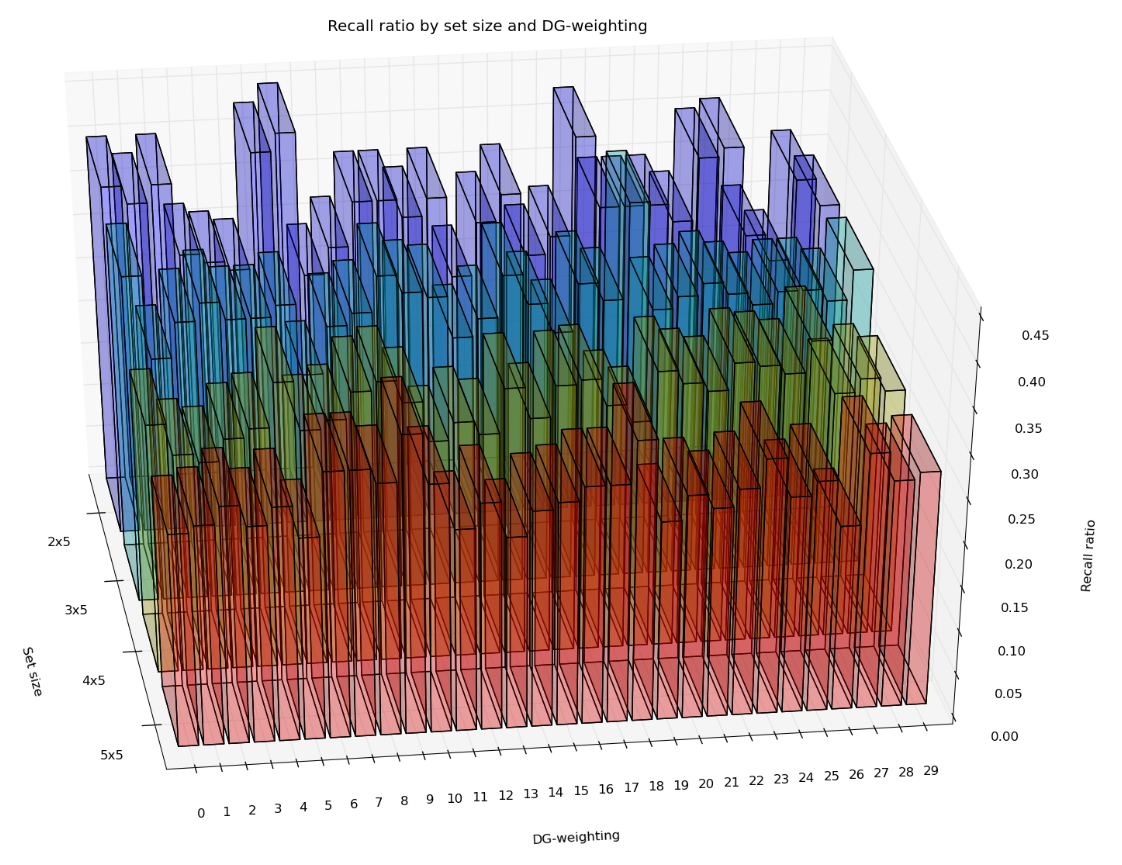
\includegraphics[width=13cm]{fig/DGWs/cut/avg_recall_ratio_by_dgw_sync_tm0_50_cut}
%     \caption{Perfect recall rate for synchronous CA3-layer neuronal updates, using a turnover rate $\tau=0.50$, and neuronal turnover between learnt subsets. It seems that using the DG-layer altogether does only slightly enhance the extraction rate of the model with the current parametrization. Furthermore, the extraction rate relative to the pattern size of perfectly recalled patterns remains fairly uniform across all training set sizes.}
%     \label{fig:avg_recall_ratio_by_dgw_sync_tm0_50}
% \end{figure}
% \begin{figure}
%     \centering
%     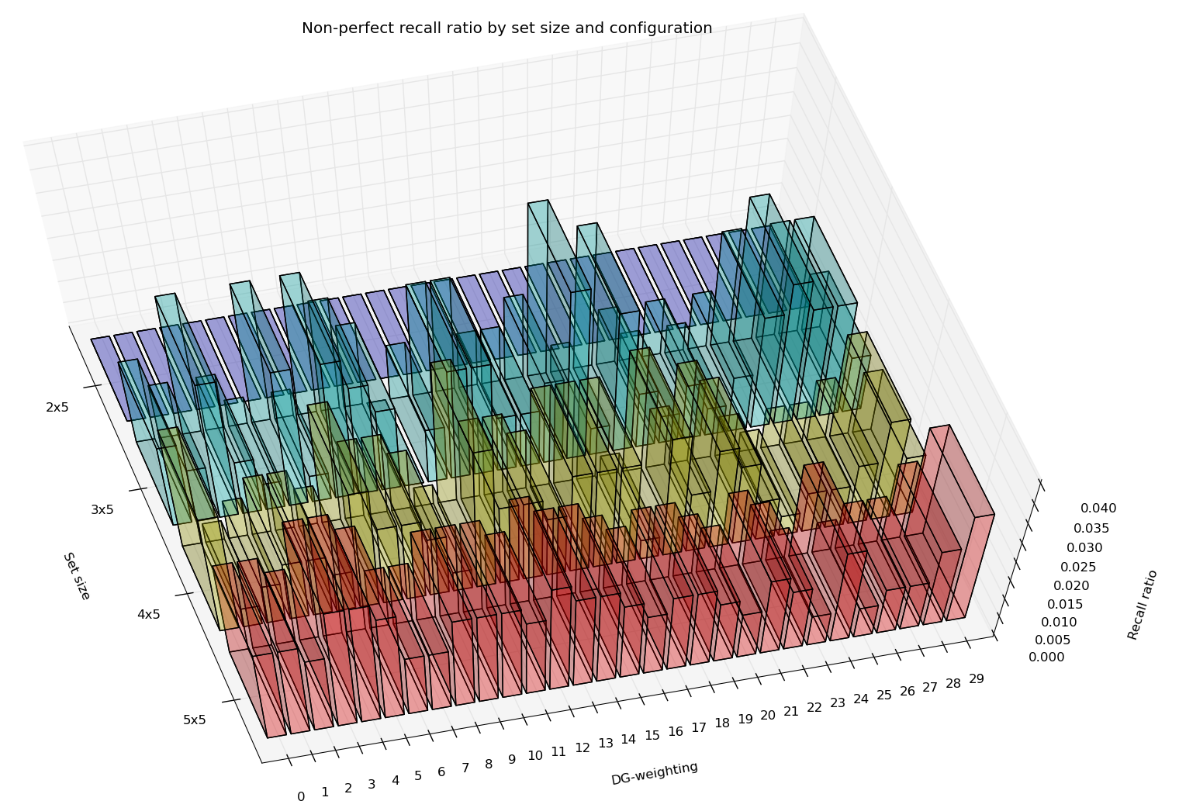
\includegraphics[width=13cm]{fig/DGWs/cut/non_perfect_recall_by_dgw_sync_tm0_50_cut}
%     \caption{Displaying the number of spuriously recalled patterns, usign the synchronous CA3 updating mode, $\tau=0.50$, and turnover between learnt sets.}
%     \label{fig:non_perfect_recall_by_dgw_sync_tm0_50}
% \end{figure}

\begin{figure}
    \centering
    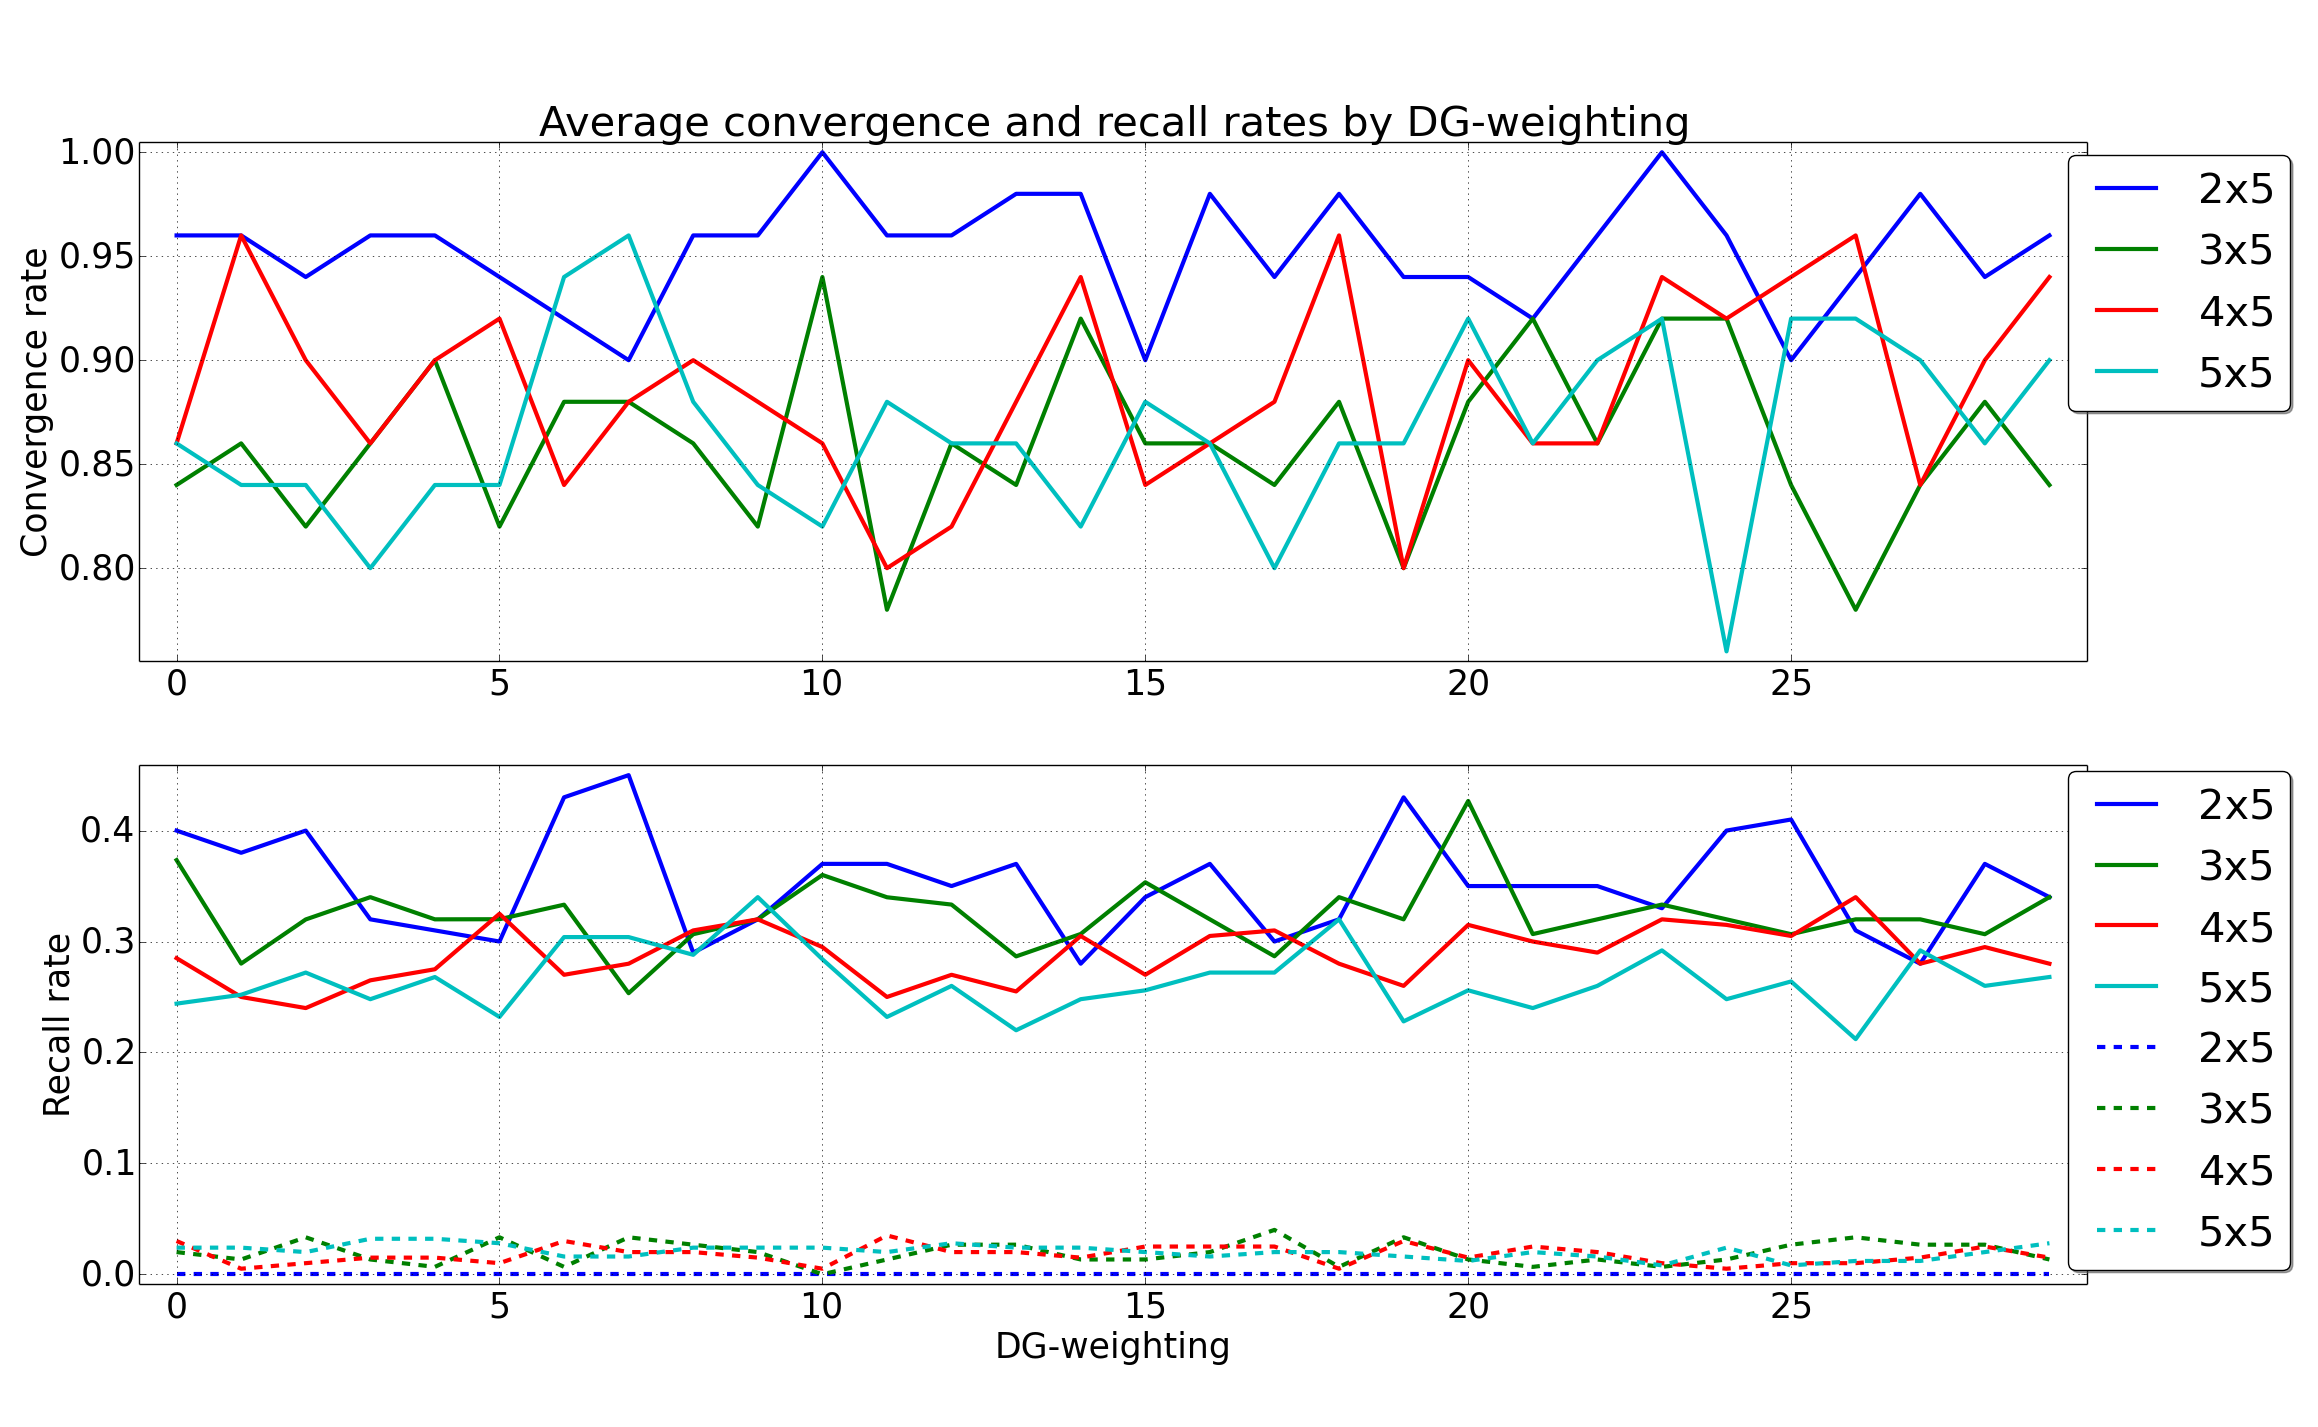
\includegraphics[width=13cm]{fig/DGWs/sync_tm0_50}
    \caption{Displaying the convergence and recall rates for the scheme of synchronous CA3-layer neuronal updates, using a turnover rate $\tau=0.50$, and neuronal turnover between learnt subsets. Note that the dashed lines in the lower subplot denote the spurious recall rates, whereas the continuous lines indicate the perfect recall rates of the corresponding set sizes. It seems that using the DG-layer altogether does not impact the extraction rate of the model with the current parametrization. Furthermore, the extraction rate relative to the pattern size of perfectly recalled patterns remains fairly uniform across all training set sizes.}
    \label{fig:sync_tm0_50}
\end{figure}

% \begin{figure}
%     \centering
%     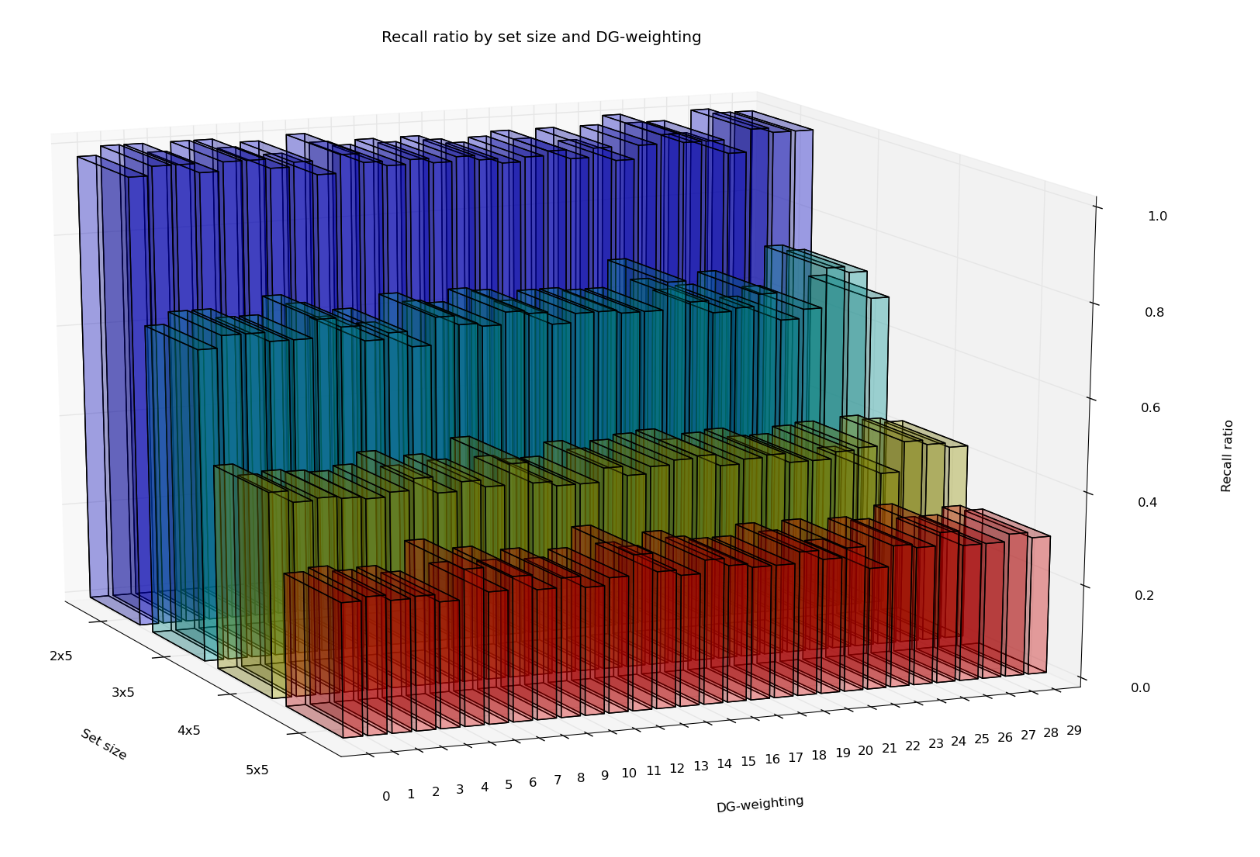
\includegraphics[width=13cm]{fig/DGWs/cut/avg_recall_ratio_by_dgw_async_tm0_50_cut}
%     \caption{Perfect recall rate for synchronous CA3-layer neuronal updates, using a turnover rate $\tau=0.50$, and neuronal turnover between learnt subsets. It seems that using the DG-layer altogether does only slightly enhance the extraction rate of the model with the current parametrization. Furthermore, the extraction rate relative to the pattern size of perfectly recalled patterns remains fairly uniform across all training set sizes.}
%     \label{fig:avg_recall_ratio_by_dgw_async_tm0_50}
% \end{figure}

% \begin{figure}
%     \centering
%     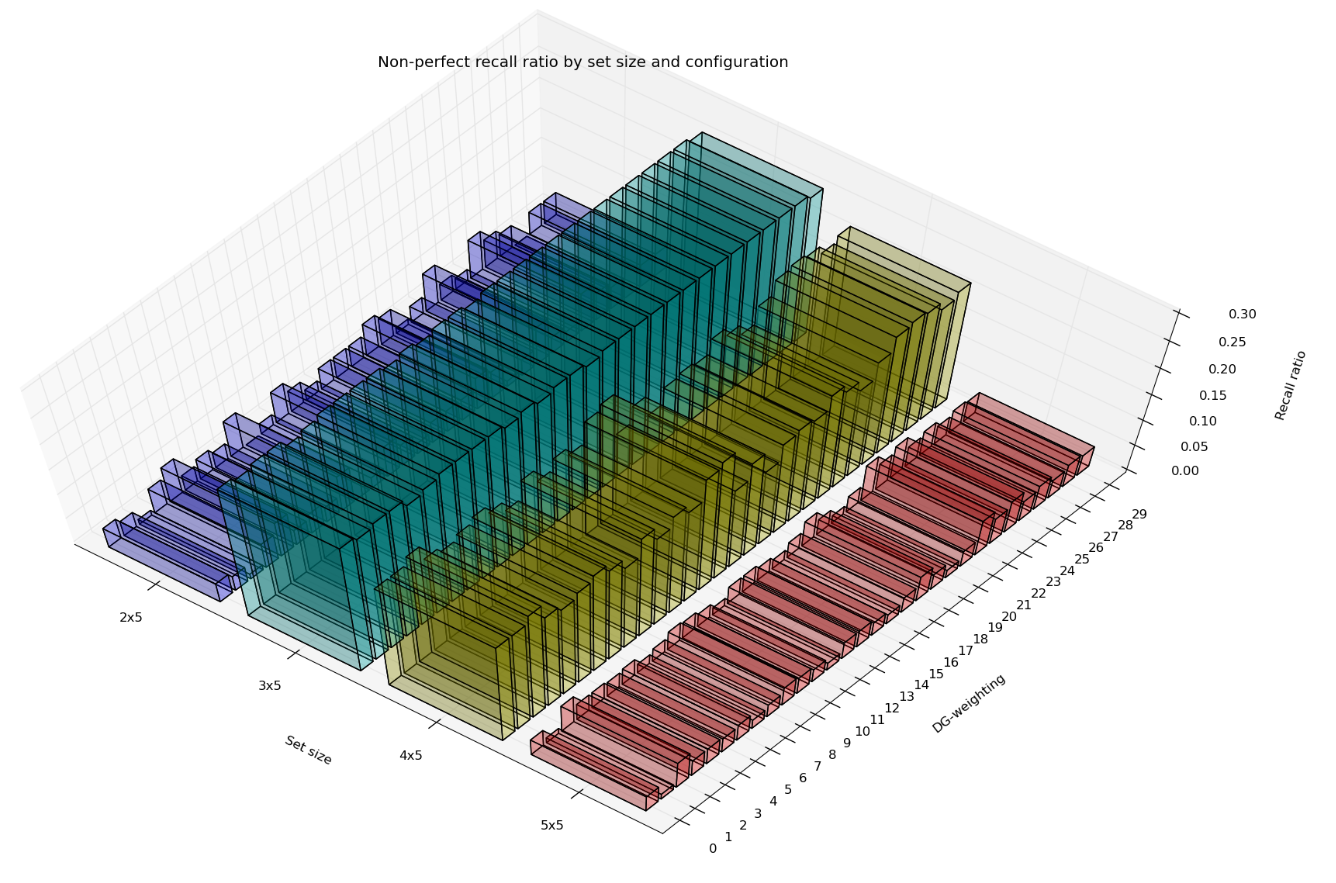
\includegraphics[width=13cm]{fig/DGWs/cut/non_perfect_recall_by_dgw_async_tm0_50_cut}
%     \caption{Displaying the number of spuriously recalled patterns, usign the synchronous CA3 updating mode, $\tau=0.50$, and turnover between learnt sets.}
%     \label{fig:non_perfect_recall_by_dgw_async_tm0_50}
% \end{figure}

\begin{figure}
    \centering
    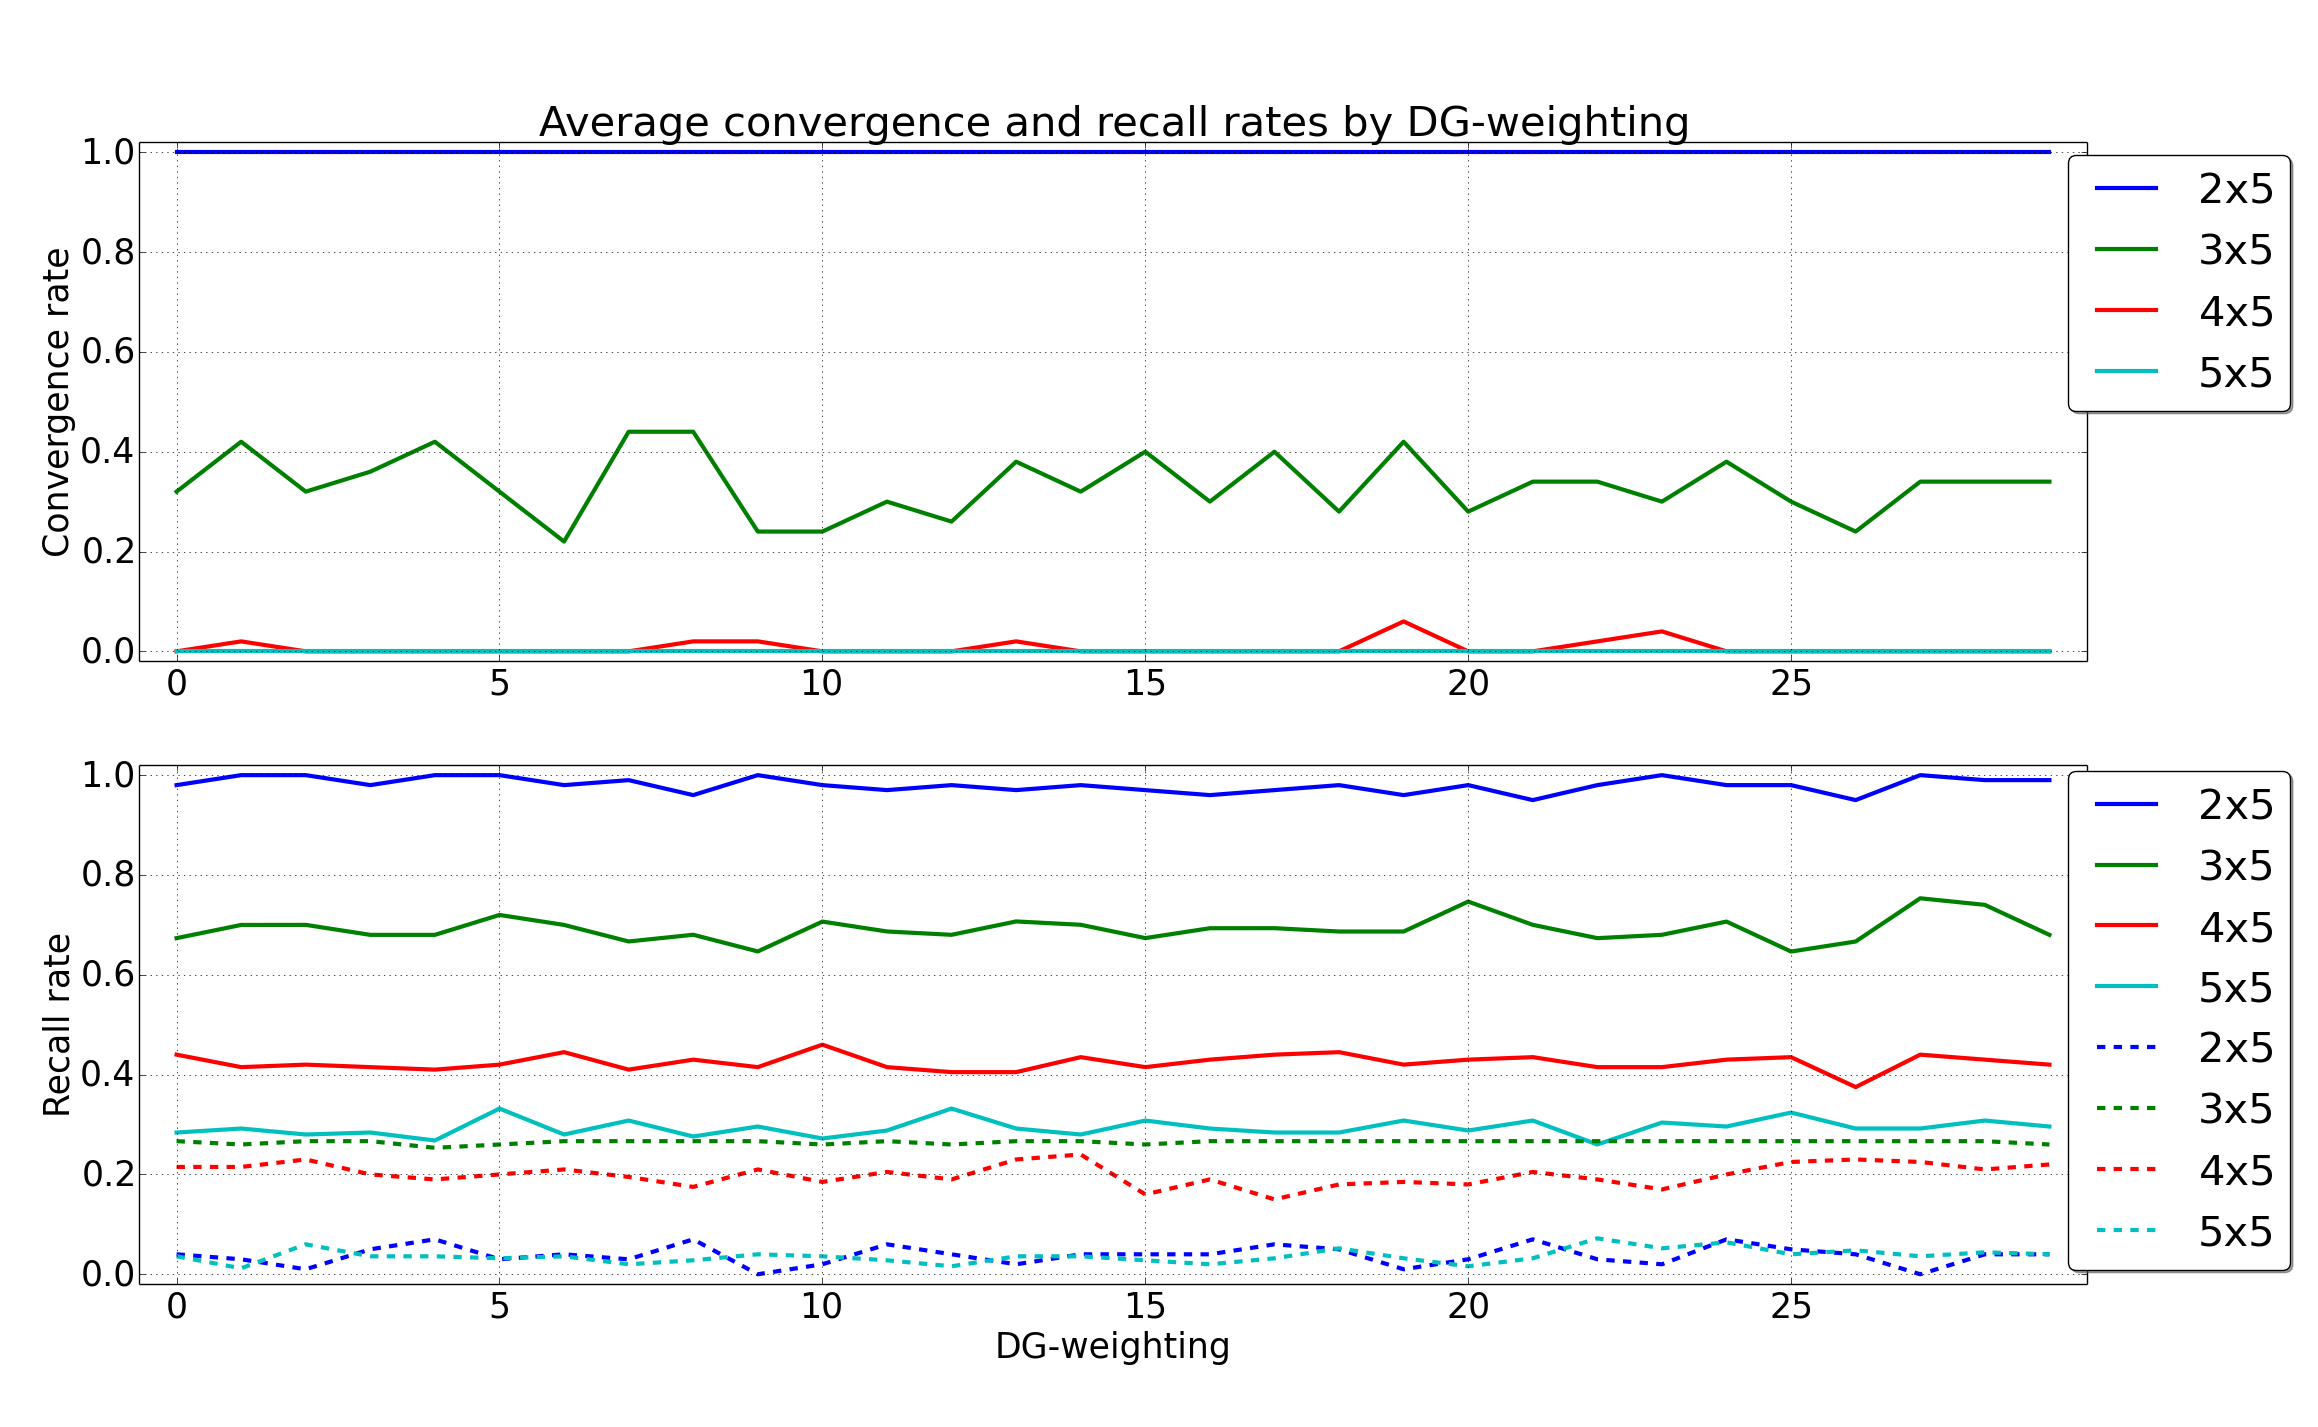
\includegraphics[width=13cm]{fig/DGWs/async_tm0_50}
    \caption{Displaying the number of spuriously recalled patterns, using the asynchronous CA3 updating mode, $\tau=0.50$, and turnover between learnt sets. Interestingly, in the cases where convergence is near perfect and where convergence is very poor, no spurious patterns are extracted.}
    \label{fig:async_tm0_50}
\end{figure}

Note in figure \ref{fig:sync_tm0_50} that the perfect recall rate is fairly equal for all training set sizes. This may indicate that either few basins of attractions are formed, or that only few basins are reached during chaotic recall. As the model converges in nearly 100 \% of the cases, the latter is likely to be the case. Figures for synchronous CA3-layer updating, using turnover for every set iteration, with the neuronal turnover rate $\tau=0.04$, are included in appendix E. These figures are very similar to the ones attained for the scheme using turnover for every new set only, with $\tau=0.50$.

As for the DG-weighting itself, note that there seems to be no significant correlation nor performance gain with the DG-weighting. Therefore, pattern separation from the DG-CA3-connections seem to be largely unsuccessful during recall.
Note also that discarding the activity of the layer altogether during learning does not result in significantly worse model performance, which strengthens the hypothesis that the activity of the DG-layer is unsuccessful in heavily influencing the activity of the CA3-layer. 
This may be the case due to the synchronicity in the CA3-updates. 
However, when looking at the figures for the asynchronous CA3 updating schemes, both schemes generate very similar figures, the turnover mode with turnover for between every learnt subset only being the included figure as for the synchronous scheme, whilst the latter is contained in appendix E.
Interestingly, near perfect and poor convergence results in approximately no spuriously recalled patterns. This could suggest that the two other set sizes partly successfully separate patterns. However, when considering that the convergence rate drops rapidly when increasing the training set size, this suggests that pattern separation is unsuccessful, as introducing more patterns (and more overlap) results in very poor model performance. Furthermore, the recall rates for both perfect recall and spurious recall are highly correlated with the convergence rate, which strongly suggests that introducing asynchronicity may increase the perfect recall rate, but does so highly due to increasing the randomness and spuriously recalled patterns. Furthermore, the model performance for the largest set size is so poor that is may only learn to recall one to two patterns for set sizes 4x5 and 5x5. These basins of attraction are the only ones that the model may converge towards, also strengthening the claim that the model capacity is reduced to one or two patterns due to unsuccessful pattern separation.


% ======================= turnover rates ========================
\subsection{Experiment 3: Neuronal turnover rate}

As the neuronal turnover rate may directly impact the model's separation capabilities, and is shown to be correlated with model performance by \citep{Hattori2014}, I here investigate model convergence, perfect recall rate and spurious pattern recall rate, here defined as non-perfect pattern recall, relative to the turnover rate for several model schemes, see table \ref{table:turnover_schemes}. These experiments may elucidate why pattern separation was unsuccessful for all of the DG-weightings in the former experiments.

\begin{table}[]
\centering
\caption{Showing the setup schemes used for investigating the impact of the neuronal turnover rate on model performance. Note that neuronal turnover modes 0, and 1, correspond to turnover between every learnt set, and turnover for every training iteration, respectively.}
\label{table:turnover_schemes}
\begin{tabular}{|c|c|c|}
\hline
\multicolumn{3}{|c|}{Setup}                               \\ \hline
CA3 updating mode & DG-weighting & Turnover mode        \\ \hline
Async             & 1            & 0                      \\ \hline
Async             & 25           & 0                      \\ \hline
Async             & 1            & 1                      \\ \hline
Sync              & 1            & 0                      \\ \hline
Sync              & 25           & 0                      \\ \hline
Sync              & 25           & 1                      \\ \hline
\end{tabular}
\end{table}

Interestingly, the asynchronous updating mode and dentate granule neurons weighting seemed to to have no impact on model performance, nor did varying the turnover rate, $\tau$.

\begin{figure}
    \centering
    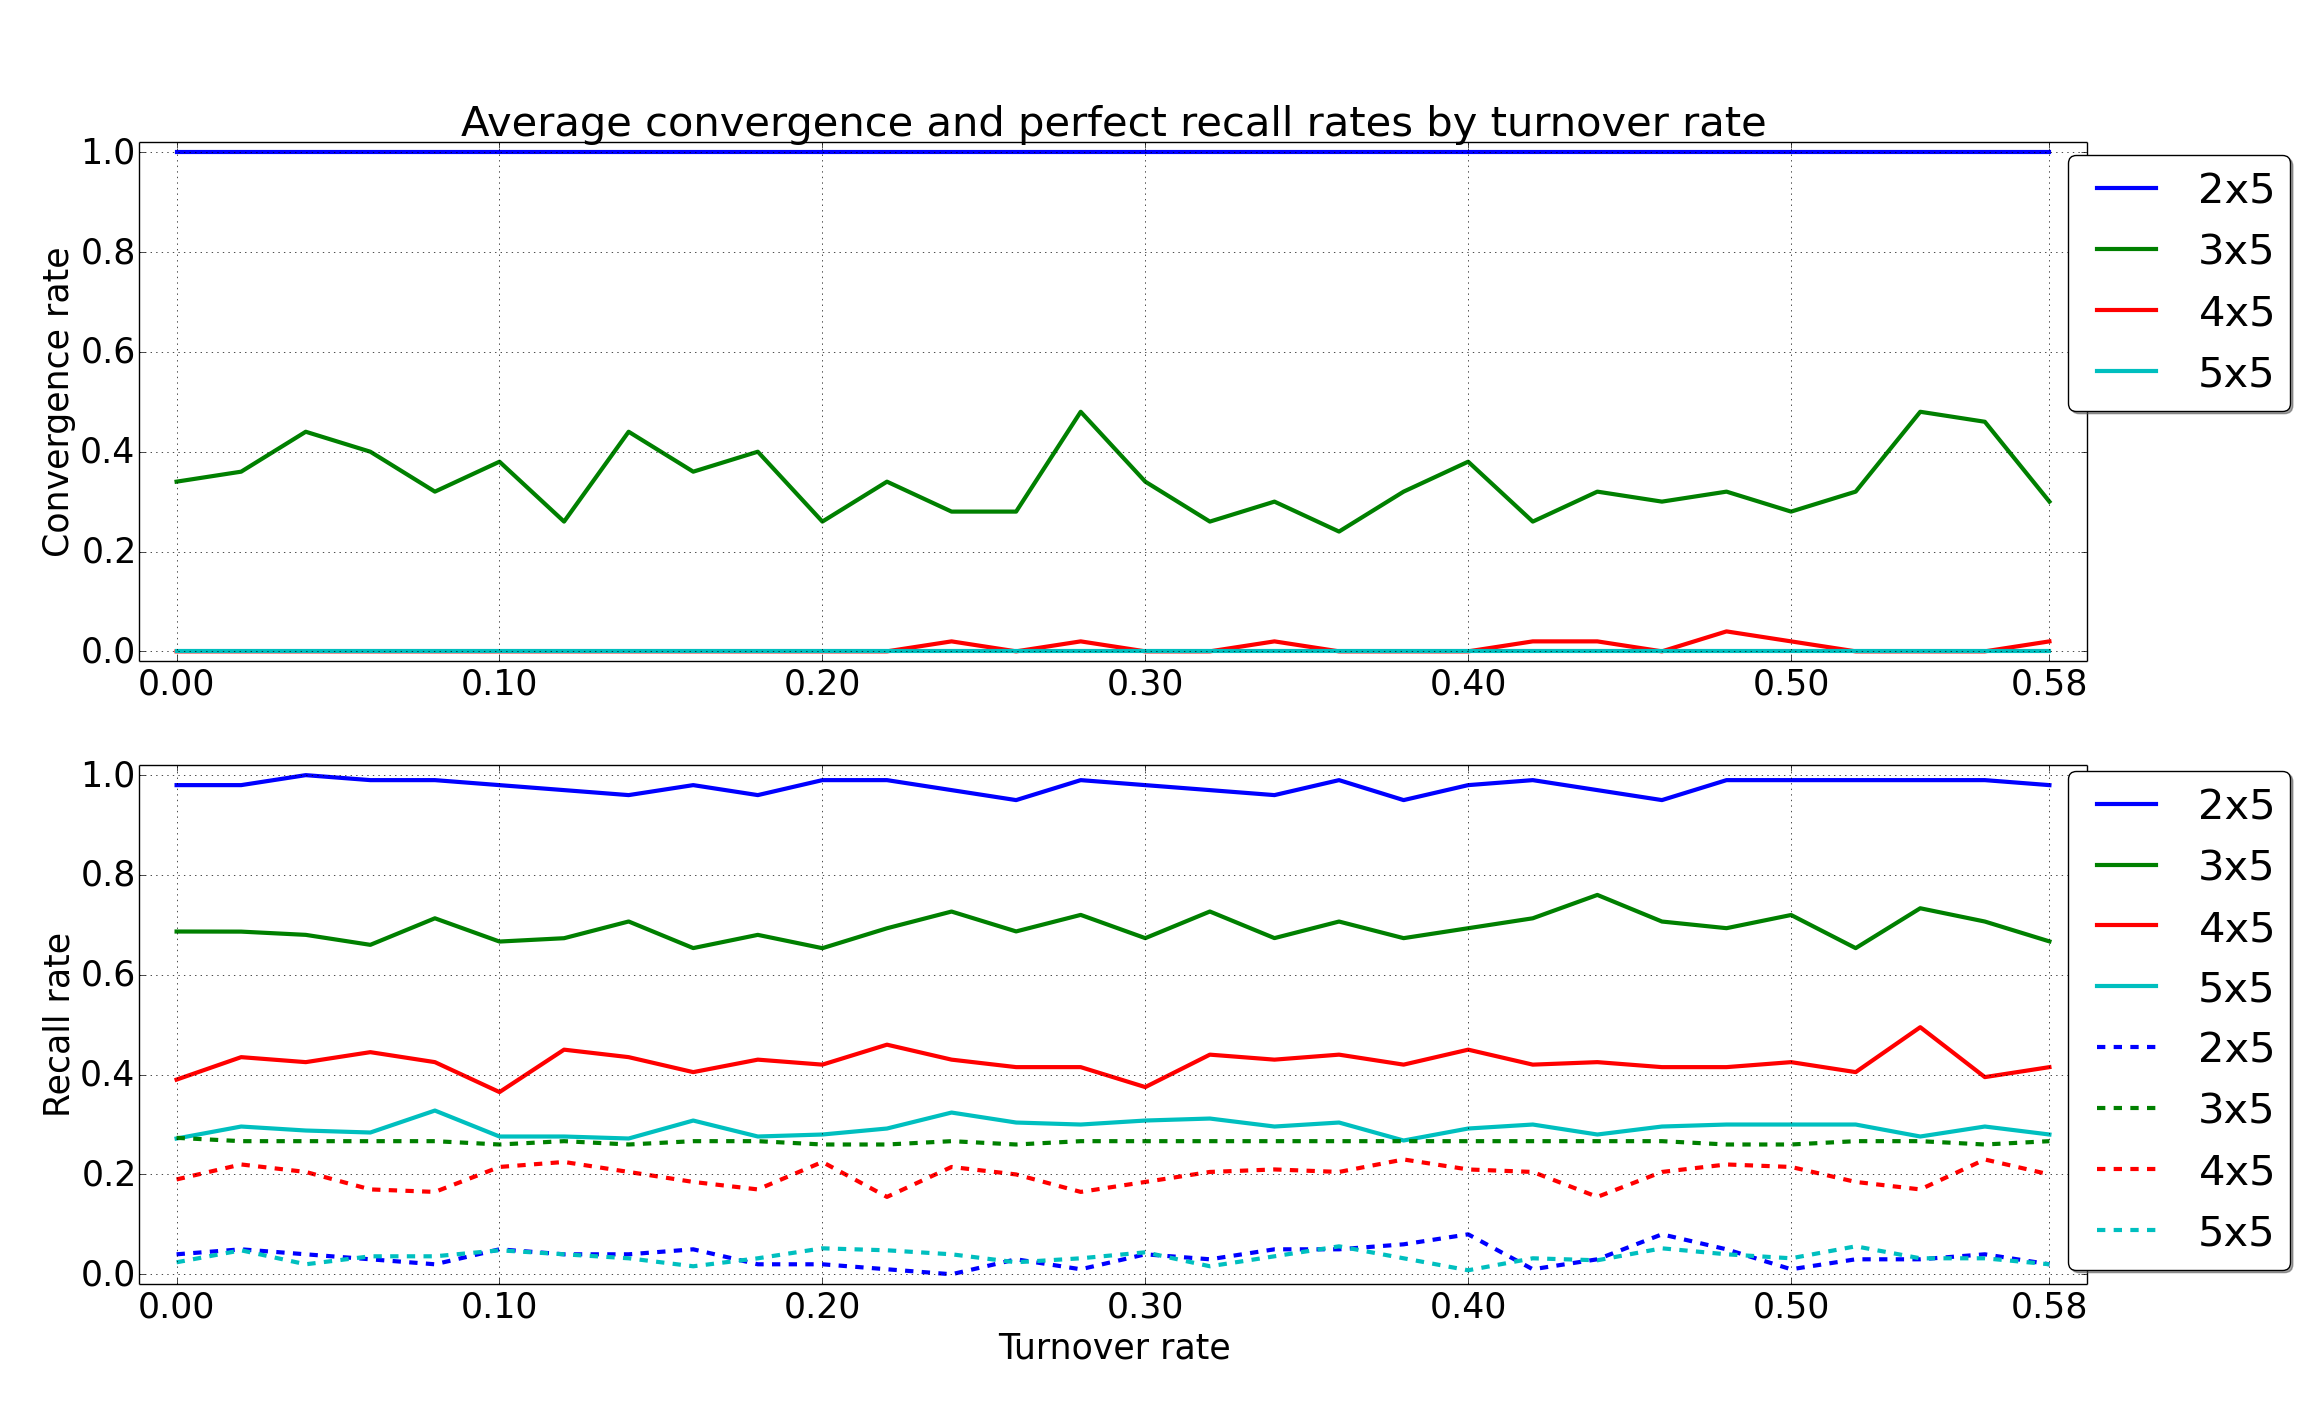
\includegraphics[width=13cm]{fig/turnover_rates/async_tm0_dgw1}
    \caption{Displaying the average convergence- and perfect and spurious recall rates by the neuronal turnover rate. In these figures the model employs asynchronous CA3 neuron-updates, with neuronal turnover being performed between every learnt training subset. Note that the perfect recall rate seems unaffected by a changing turnover rate.
    Average convergence by neuronal turnover rate, for asynchronous CA3 neuronal updating, and turnover between every learnt training (sub-)set. Note that convergence seems unaffected by a changing turnover rate.}
    \label{fig:async_tm0_dgw1}
\end{figure}

Figure \ref{fig:async_tm0_dgw1} raises the question of whether the model contains any issues related to the DG-layer, as the layers' parameters do not seem to affect model performance. Because highly similar results were attained for all three neuronal turnover configurations when using asynchronous CA3-layer updating, figures for the two remaining asynchronous model schemes are contained in appendix E.
It may be that the asynchronous CA3-layer updating scheme introduces a certain robustness to the model, seeing that permuting and re-instantiating a large number of the EC-DG and DG-CA3 synapses for every training set iteration does not reduce the model performance. 
However, the convergence rates indicate poor convergence in all scenarios. Furthermore, when investigating the figures (\ref{fig:sync_tm0_dgw25}, \ref{fig:sync_tm1_dgw25}) for synchronous CA3-neuron updating, neuronal turnover rate does in fact positively impact the perfect recall rates of the model when the DG-weighting is set to $25$.

\begin{figure}
    \centering
    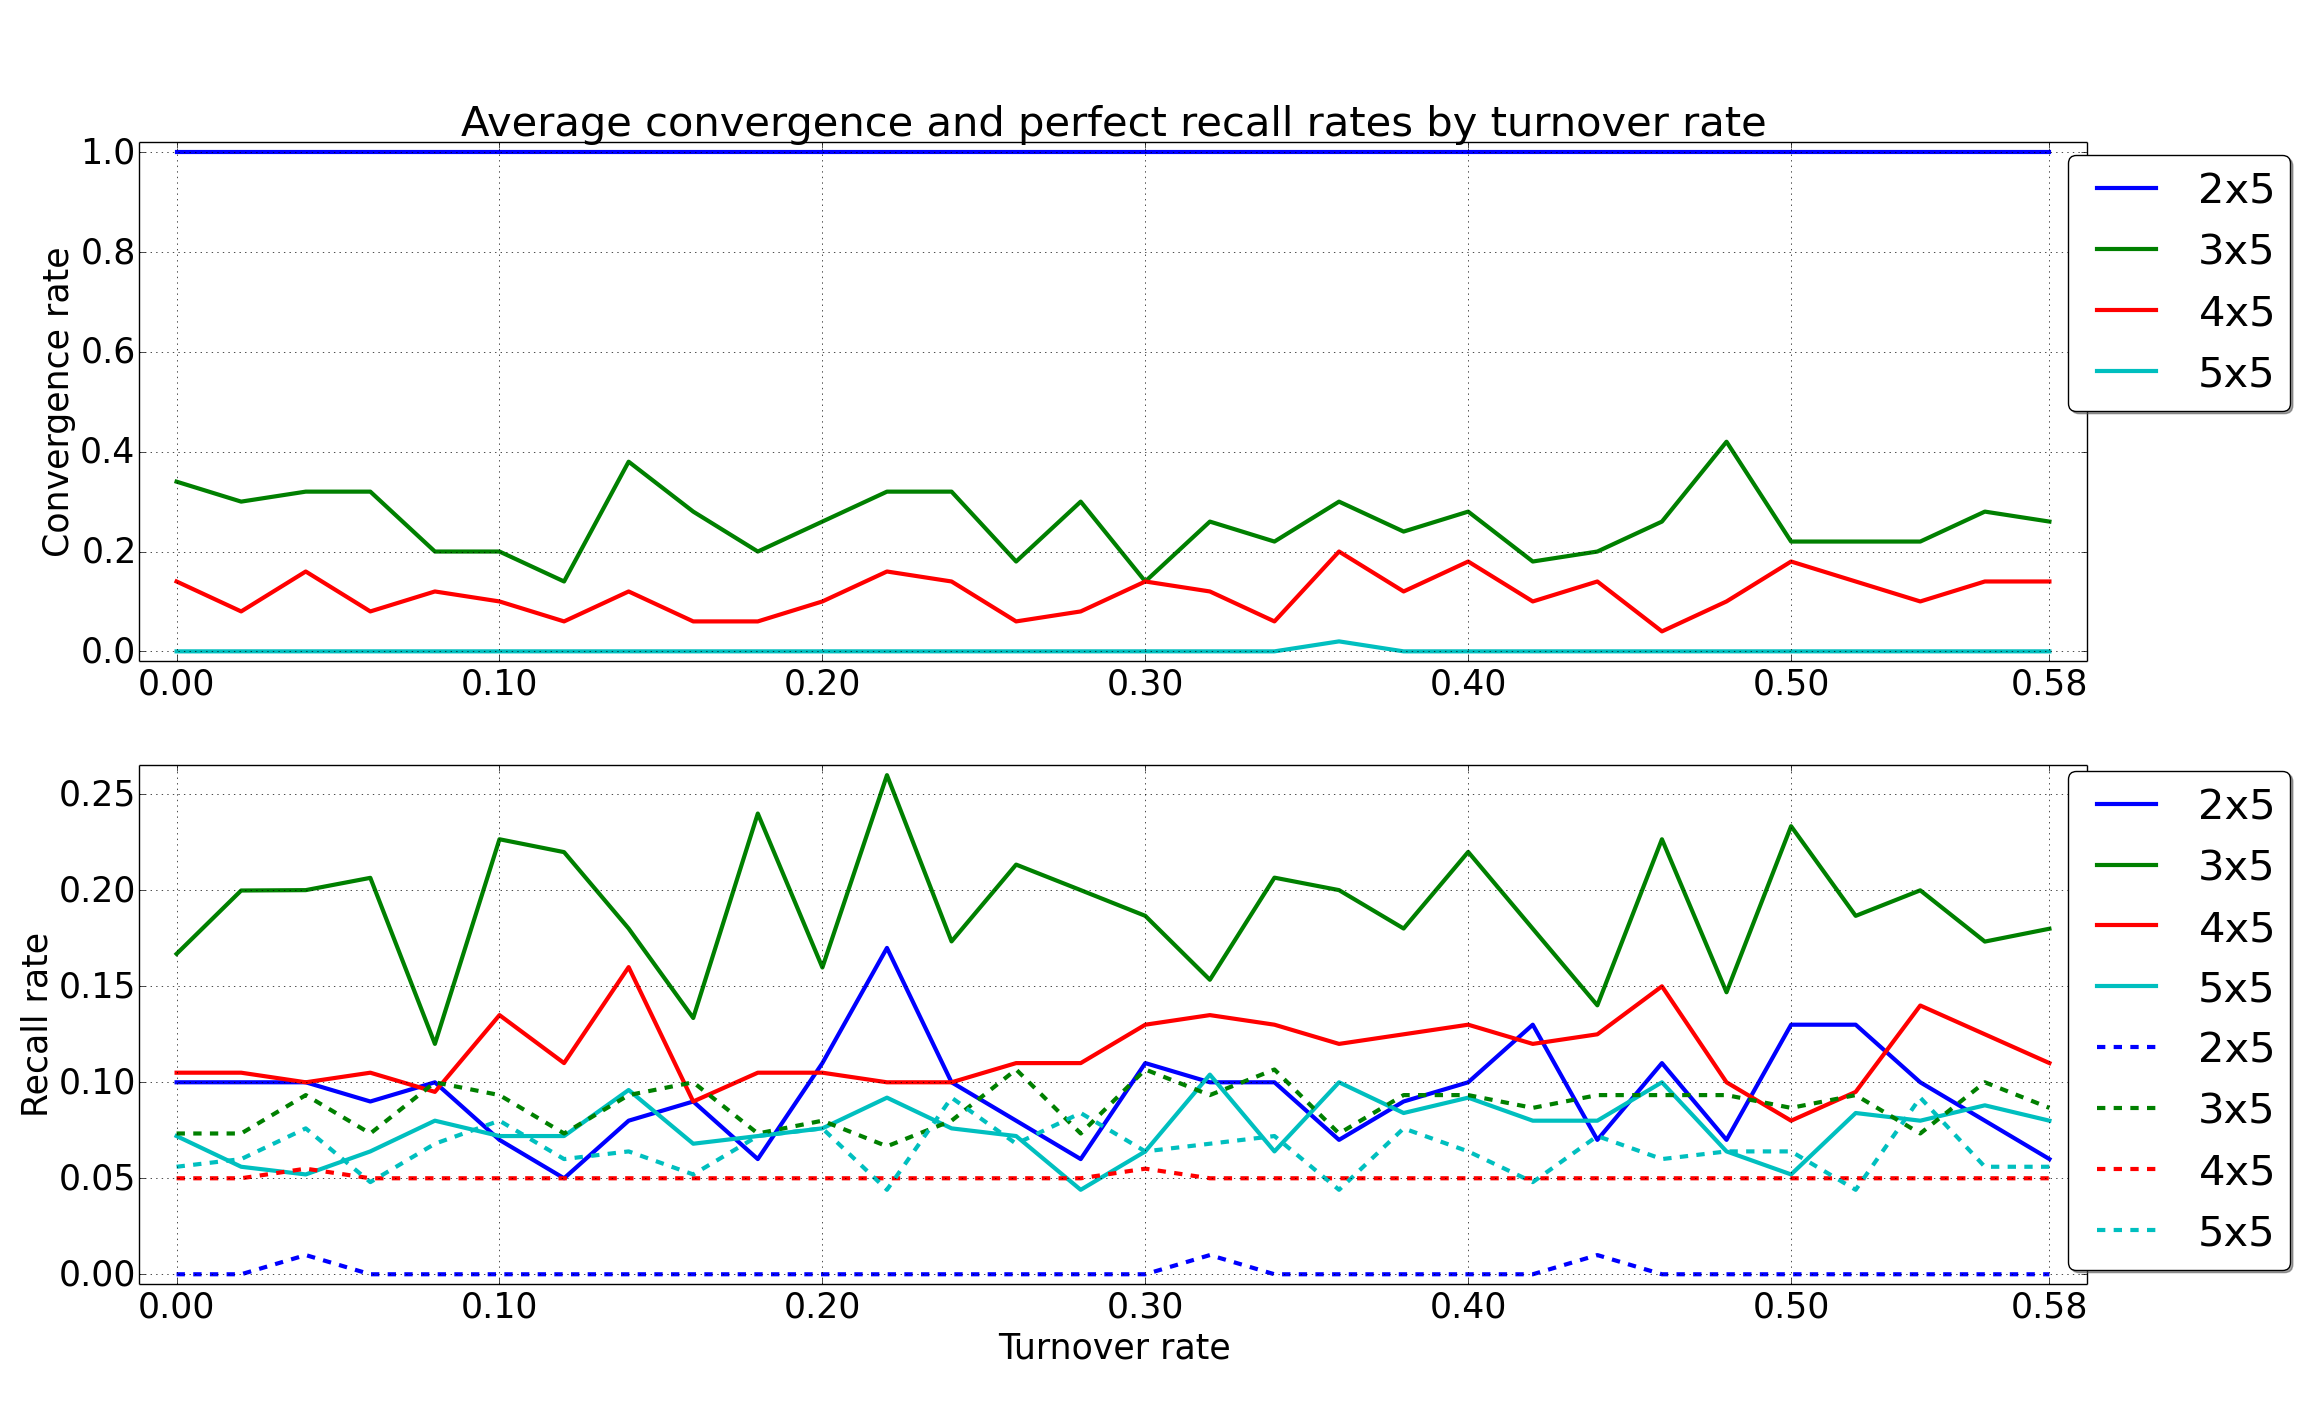
\includegraphics[width=13cm]{fig/turnover_rates/sync_tm0_dgw1}
    \caption{Illustrating the average model convergence and recall rates by neuronal turnover rate for synchronous CA3-layer updating, using a DG-weight coefficient of 1, and neuronal turnover between every learnt training subset. As the model seems to largely fail to converge for any set size other than 2x5, this may indicate that pattern separation is unsuccessful, which would also explain why changing the neuronal turnover rate does not affect the model performance in figure \ref{fig:async_tm0_dgw1}.}
    \label{fig:sync_tm0_dgw1}
\end{figure}

Model convergence is not attained in the synchronous CA3 neuronal updating scheme when a DG-weighting of 1 is employed, with the perfect recall rate remaining poor. This suggests that the model is both unable to separate the patterns for the correct input patterns during learning and recall when the DG-weighting is 1.
Note that when increasing the DG-weighting to 25, the model converges for 80-100 \% of the training patterns, irrespective of set size. Further, this results in perfect recall rates of twice as high values, suggesting that increasing the connection weighting of the synapses from the DG-layer to the CA3-layer may in fact enable pattern separation during learning and chaotic recall. 
Note that the neuronal turnover rate seems uncorrelated with model performance when performing neuronal turnover between learnt subsets. Interestingly, when performing neuronal turnover for every training iteration (DG-weighting $= 25$, synchronous updating), results in the best model performance attained so far. Namely in  nearly 80 \% of the training sets from the 3x5 auto-associative training set being perfectly recalled for $\tau\in\approx[0.40, 0.58]$.
Furthermore, there is a slight increase in the recall capability during learning of the other set sizes too. It is important to emphasise that while perfect recall increases significantly for higher turnover rates, with the highest rate in the aforementioned interval; so does spurious pattern recall. While such low spurious recall rates may be acceptable, strict convergence is only attained for sufficiently low turnover rates. Interestingly, the figure suggests that rather high turnover rates may be used while not spuriously recalling patterns (such as $\tau=0.30$). Furthermore, note that some patterns are spuriously recalled for very low turnover rates. This suggests that when the turnover is too low, pattern separation is unsuccessful.
Shortly put, figures \ref{fig:sync_tm0_dgw25} and \ref{fig:sync_tm1_dgw25} elucidate pattern separation in the outlined model, demonstrating that a certain level of continuous turnover is preferable for successful pattern separation, and further suggesting that employing strongly connected synapses in the DG-CA3 pathway enables pattern separation altogether.

\begin{figure}
    \centering
    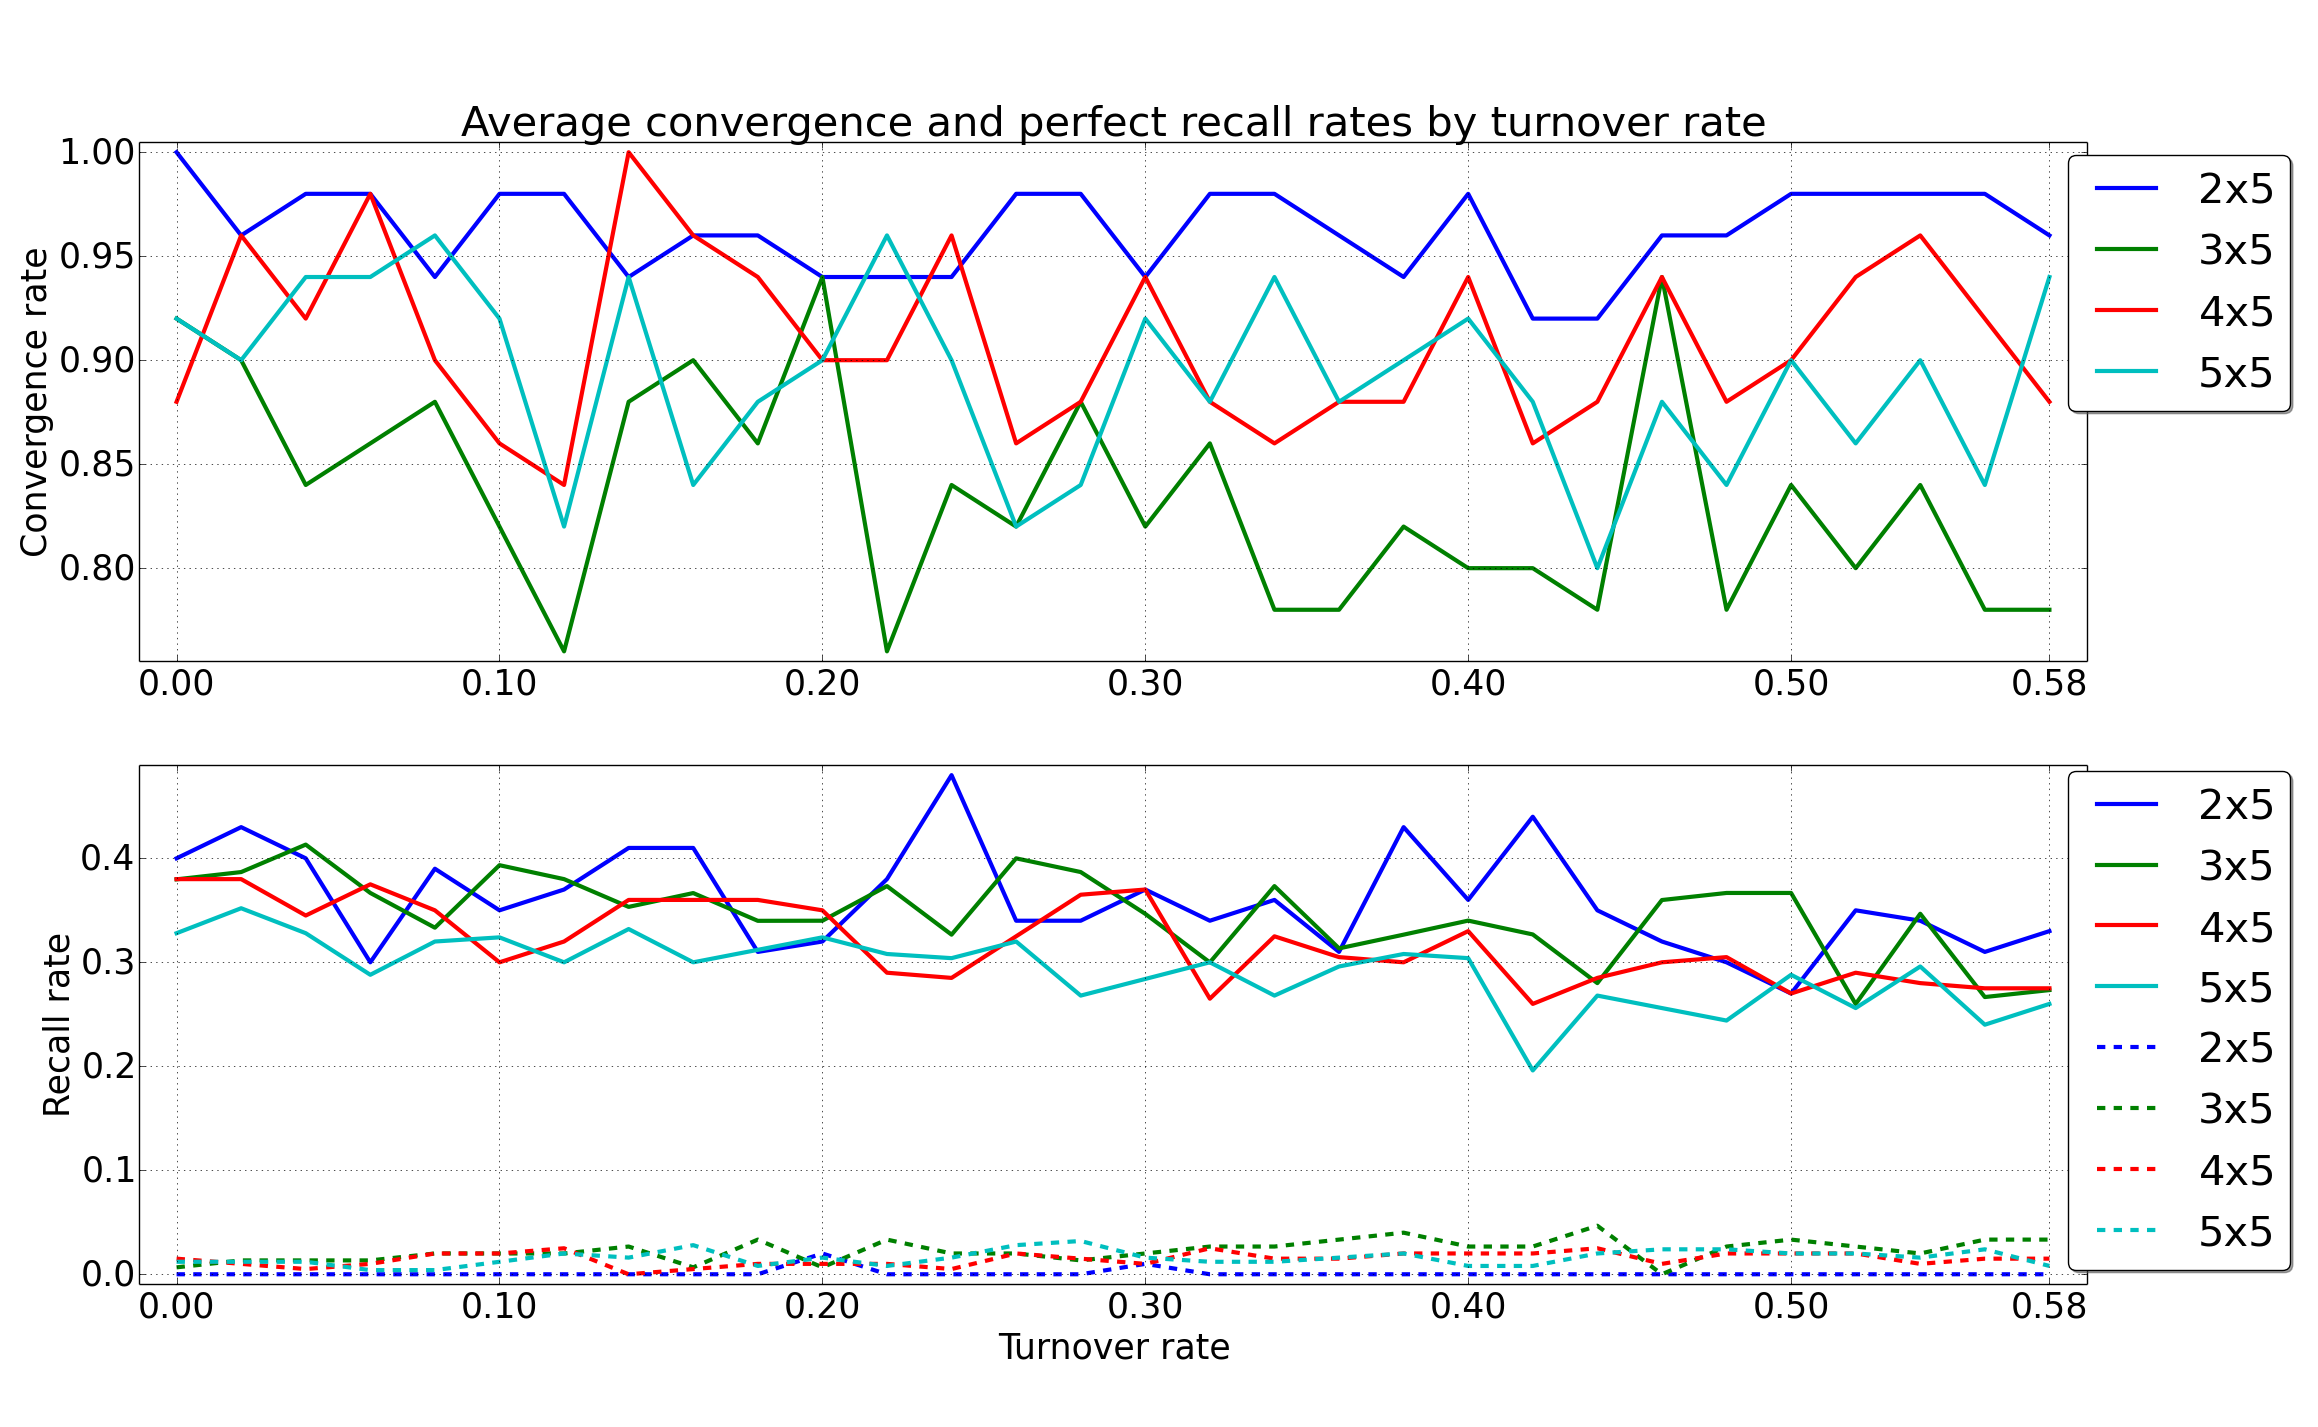
\includegraphics[width=13cm]{fig/turnover_rates/sync_tm0_dgw25}
    \caption{Presenting the average perfect recall rate for the scheme of synchronous updating, now using a DG-weighting of 25, turnover being performed for every new training subset. Note that neuronal turnover does not seem to affect model performance significantly. However, there is a slight tendency towards a worse perfect recall rate as the turnover rate grows towards 0.50.
    Convergence is attained in about 80 to 100 \% of the cases, but is not correlated with the training set size.}
    \label{fig:sync_tm0_dgw25}
\end{figure}

\begin{figure}
    \centering
    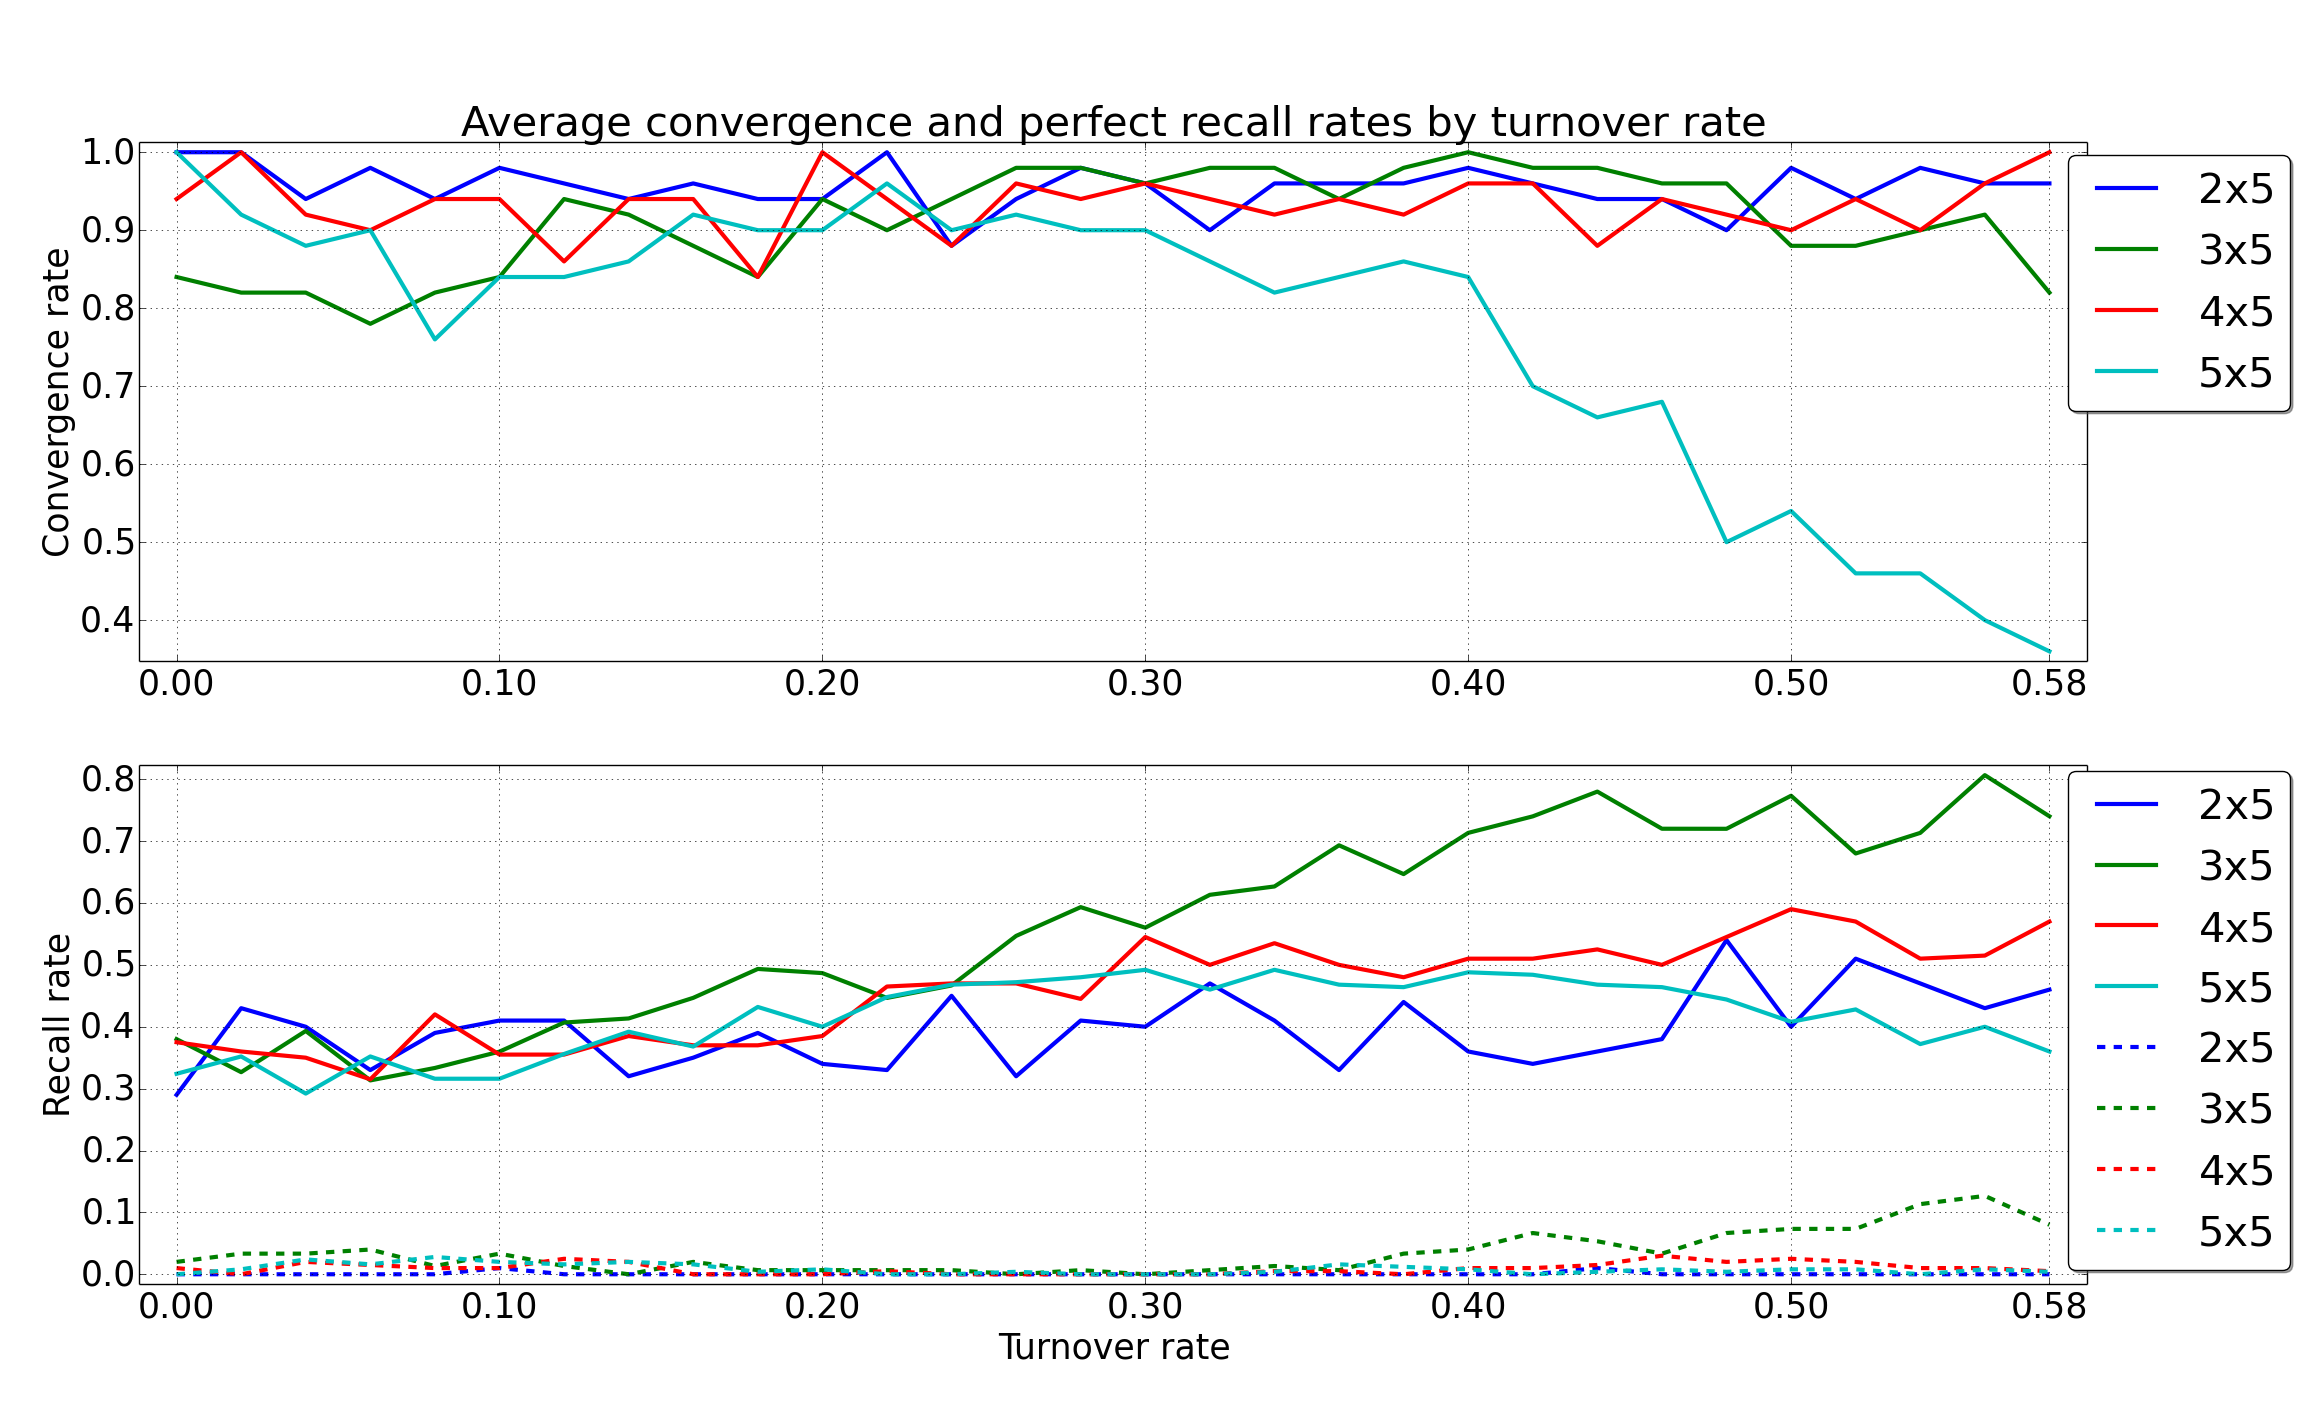
\includegraphics[width=13cm]{fig/turnover_rates/sync_tm1_dgw25}
    \caption{Showing the average perfect recall rate for the scheme of synchronous updating with a DG-weighting of 25, turnover being performed for every training iteration. Interestingly, model performance is now highly correlated with the turnover rate, when turnover is being performed very frequently.
    Convergence is attained in about 90 to 100 \% of the cases, and seems to be best for a neuronal turnover rate $\tau$ in the interval of approximately $[0, 30]$. Note that the convergence drops rapibly for the largest training set size when $\tau$ goes above this value (for $\tau \in [0.30, 0.58]$).}
    \label{fig:sync_tm1_dgw25}
\end{figure}

As asynchronous neuronal updates use the newest updated values in the CA3-layer through its recurrent connections, this may in fact introduce too much randomness in the model. One solution to this may be to introduce hardware-mediated asynchronicity through algorithmic parallelization, as this is more likely to mainly use the current neuronal values, thus largely reducing the randomness and the combinatorial explosion of the outcome space during neuronal updating and wiring. This reduction is somewhat relaxed, enabling a trade-off of yet maintaining a certain randomness to the model. Furthermore, this scheme is may be more biologically realistic, as updating in the biological brain is performed continuously and only slightly synchronously (and at different time-scales). However, both implementing and elaborating more on such a scheme remains outside the scope of this thesis.

Note the successful increase in perfectly recalled patterns for set size 3x5, but not 2x5 when increasing the neuronal turnover rate in the synchronous CA3-updating scheme using turnover for every training iteration, figure \ref{fig:sync_tm1_dgw25}. Because both patterns are successfully recalled when the correct corresponding input is present in the 2x5 training scheme, but not during recall, this suggests that one of the patterns in the 2x5 scheme covers most of the weight space, thus being the only pattern which is reached during learning. Furthermore, increasing the number of patterns also necessarily increases the need for pattern separation in order for the model to converge. Therefore, each pattern is more likely to occupy more of the weight space, thus increasing the area of its basin of attraction (i.e. the area inside which the network will converge towards the output pattern). Additionally, figure \ref{fig:sync_tm0_dgw25} demonstrates that when turnover is only performed between training sets, increasing the turnover rate only slightly decreases the perfect recall rate. This suggests that while increasing the frequency of performing turnover to every training iteration may provide the model with more randomness, expanding the model's search through learnt patterns, it only slightly improves the recall capabilities. Furthermore, expanding the search space also introduces some more spuriousness to the recall process. This provides the basis for the next experiments, where the convergence criterion is designed to be less stringent, as well as to potentially assign patterns more evenly in the model's weight space.

% ======================= exposure schemes ========================
\subsection{Experiment 4: Relaxed convergence criterion and various exposure schemes}

Because the results presented above in experiments 1-3 indicate issues related to chaotic recall, these experiments investigate how reformulating and relaxing the convergence criterion may impact model behaviour. Convergence is now considered to be attained once a static number of training or recall iterations have been performed. In this experiment the number of iterations is set to 15, based on empirical data from previous experiments. Although the model is shown to be capable of one-shot learning in the low-level demonstration contained in the first parts of this chapter, convergence is only attained in less than 15 training iterations for set size 2x5 in the introductory experiments using the stringent convergence criterion (of stable output for three recall iterations). On average, the synchronous CA3 updating mode converged in 2-3 training iterations, which demonstrates a clear one-shot learning capability, while the in the asynchronous mode it converged in on average about 7 iterations for training set size 2x5. 
%
% Interestingly, these ranges are very similar to those thought to be required (approximately) for human subjects to learn new training sets \citep{Rolls1998chpt6} [double-check].
Nevertheless, as the set size grows larger, i.e. 3-5 per subset, the number of required training iterations grows slightly larger than 15 for the synchronous CA3 updating mode (approximately 20 for the remaining set sizes), and linearly towards 50, i.e. no convergence at all for the asynchronous CA3 updating mode.
While convergence thus may not be attained for 15 training iterations according to the previous learning criterion, the model will definitely have had time to be completely exposed to the new training subset, adapting its weights accordingly (to the set). Furthermore, 15 iterations is also more than sufficient in order to have former short-term memory diminish, as may be seen in the low-level example figures contained in appendix E.
What I wish to investigate in this experiment are the trends that may arise under a more constant training scheme. Even though convergence is not strictly attained, the number of iterations does allow for learning pattern associations. Furthermore, exposing the model to a constant and uniformly distributed continuous flow of patterns is more likely to generate trends that are representative of model behaviour, both during recall and learning. As such, observing trends for a more static scheme may ameliorate the unsuccessful chaotic recall that is observed under the more stringent chaotic recall scheme and convergence criterion. Thus, observed trends may in fact provide a better picture of the model behaviour, and the observed trends may potentially help further illuminate the research questions, as well as the pattern separation aspects related to synchronicity and neuronal turnover that remains slightly obscure from previous experiments and results.

% \subsubsection{Local training set exposure}

\begin{figure}
    \centering
    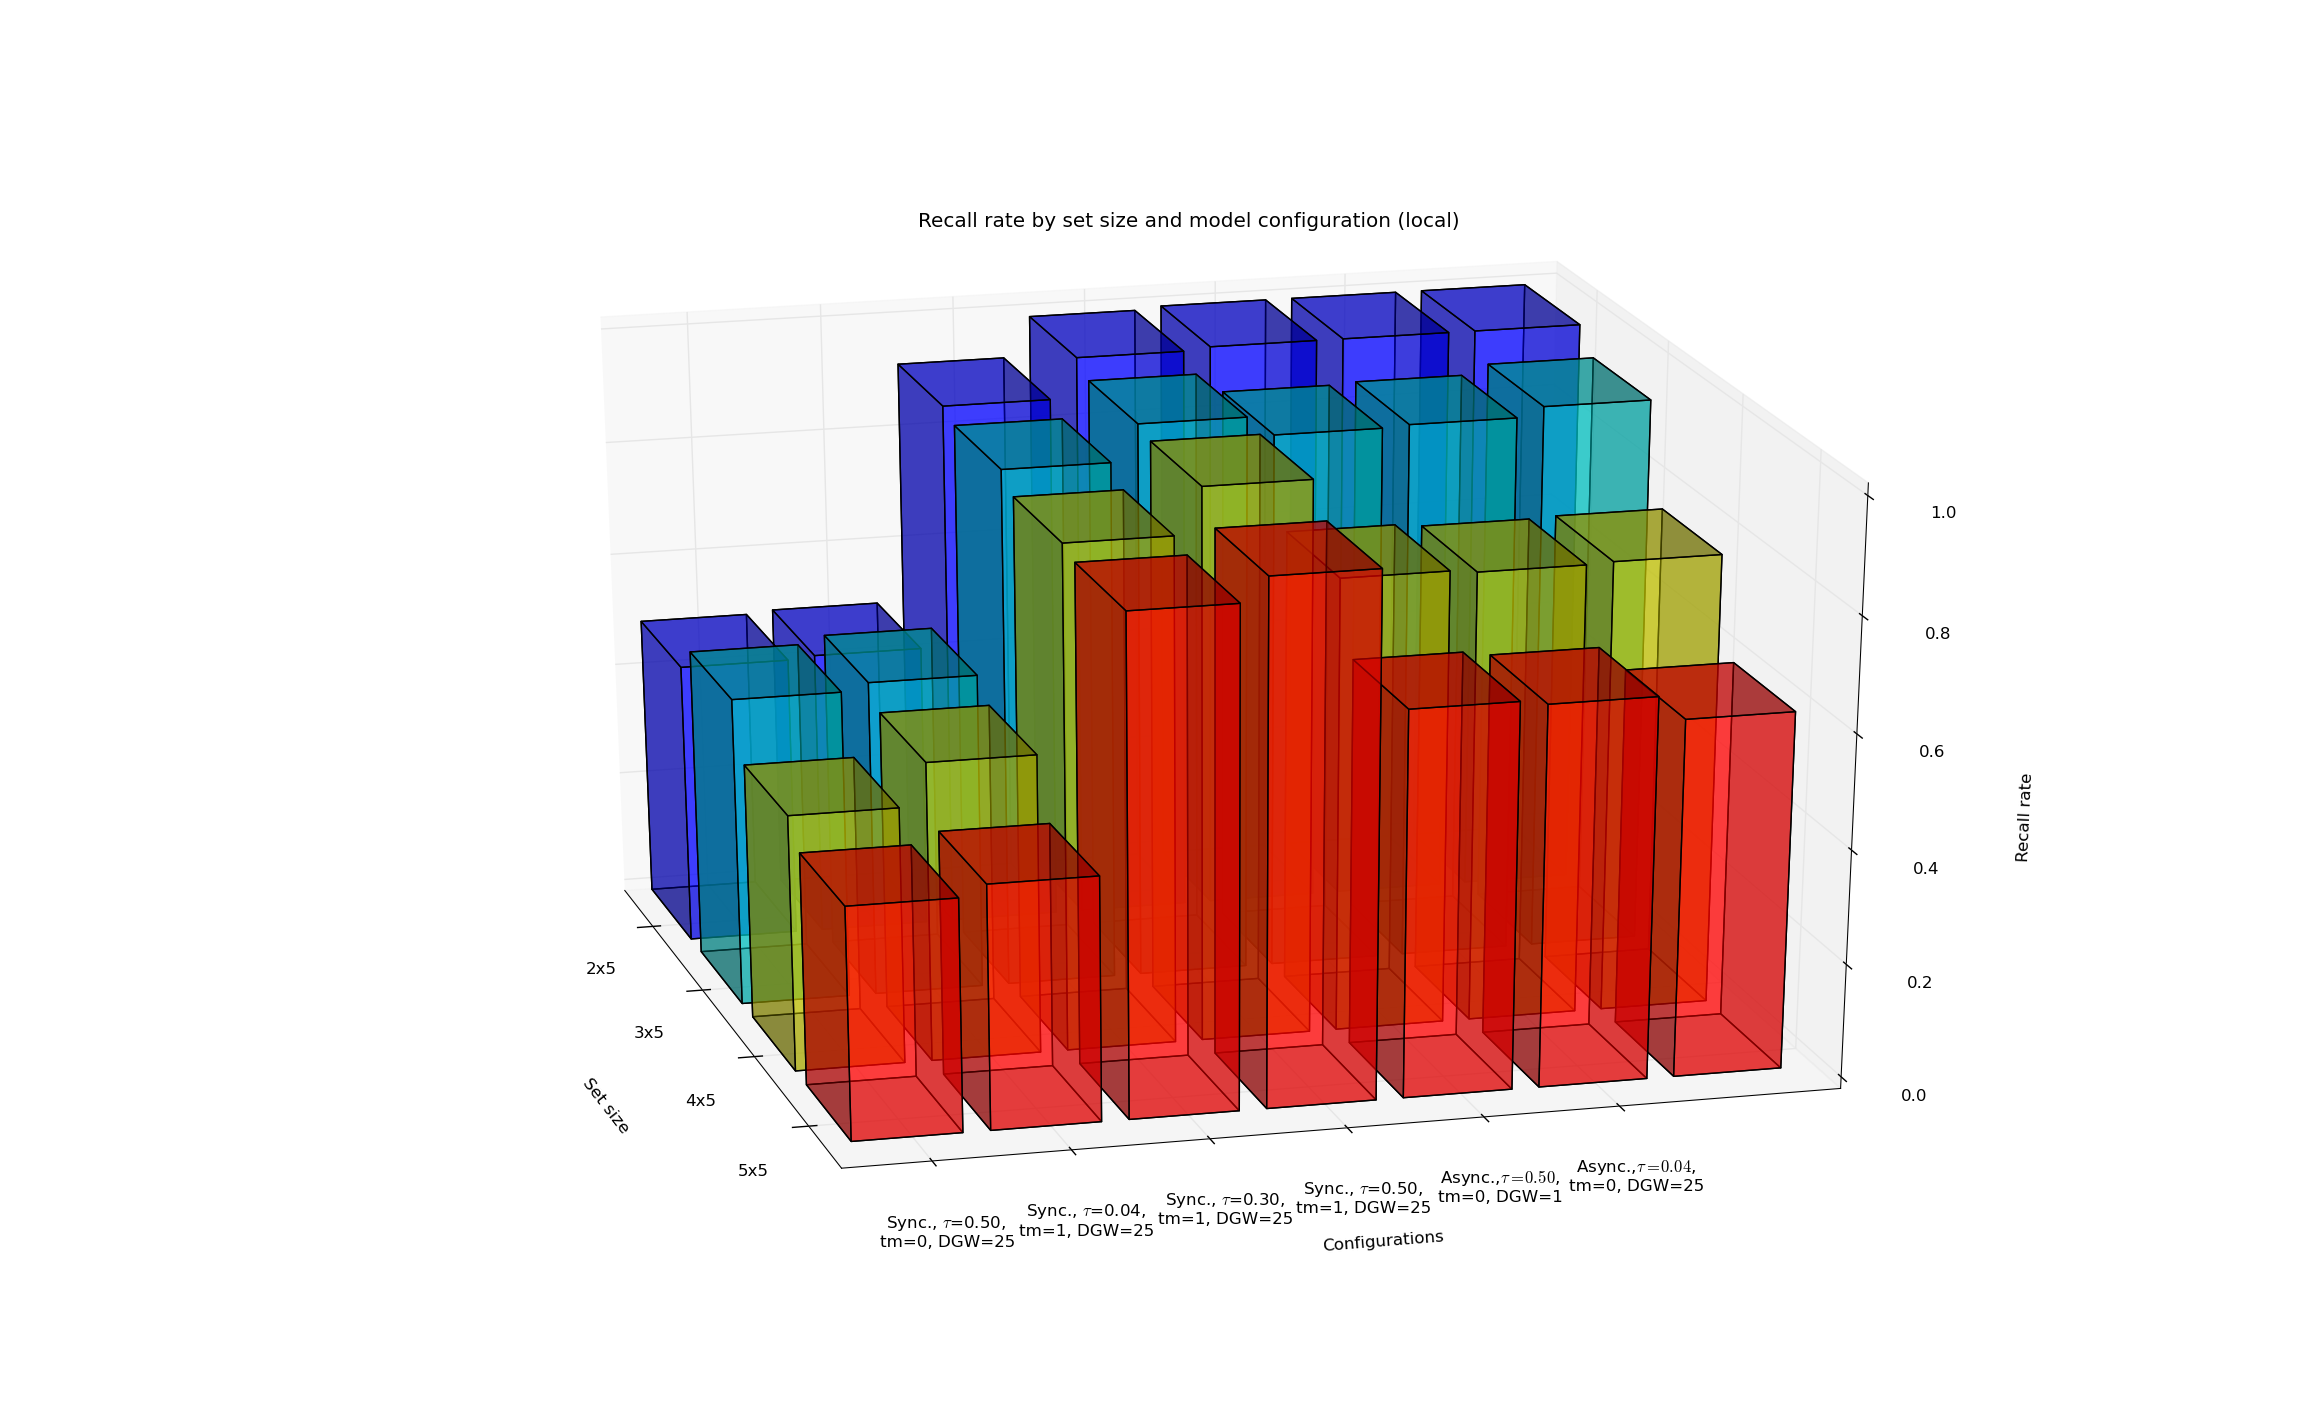
\includegraphics[width=13cm]{fig/i-iters/local-recall}
    \caption{local recall sync, async}
    \label{fig:local-recall}
\end{figure}

\begin{figure}
    \centering
    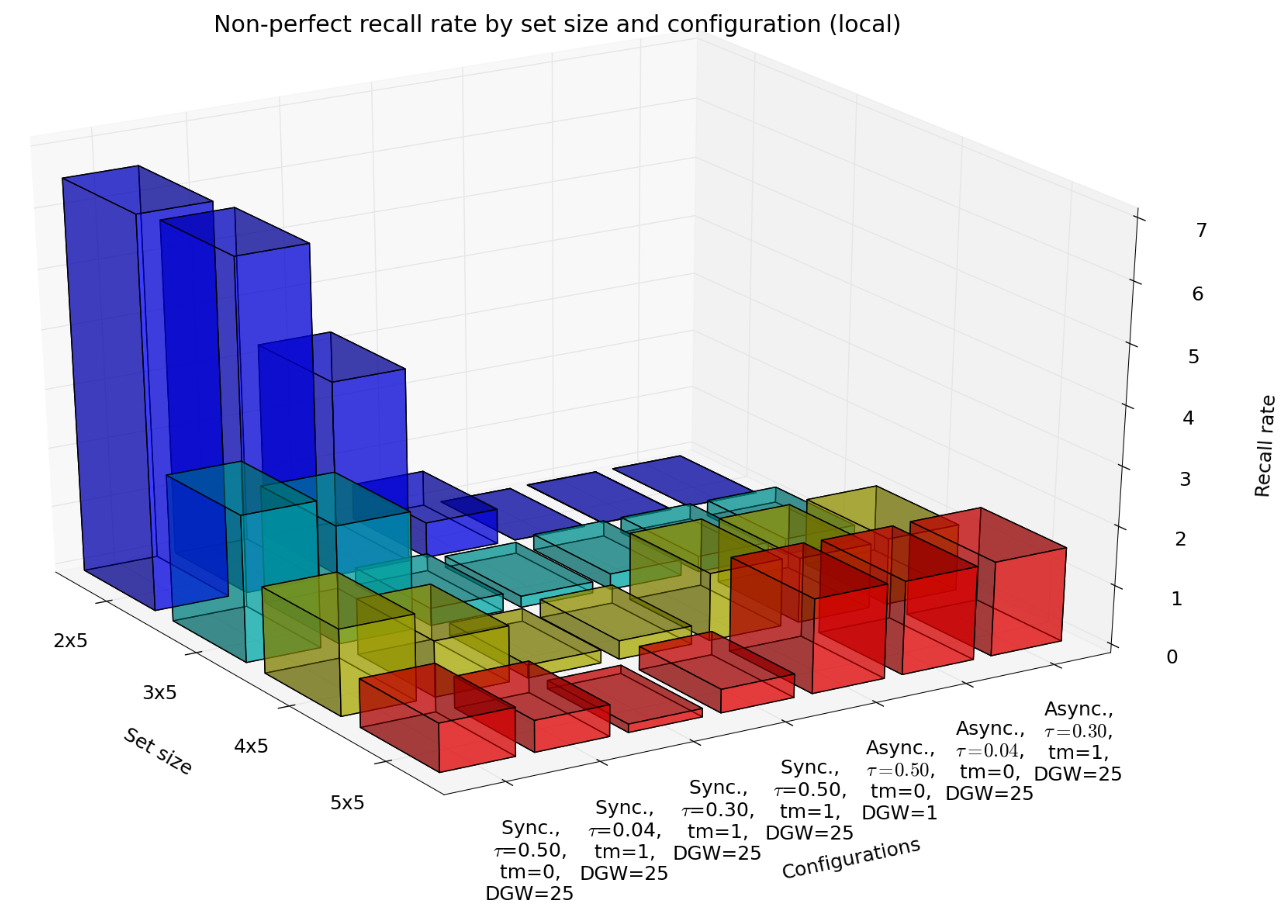
\includegraphics[width=13cm]{fig/i-iters/local-recall-spurious}
    \caption{spurious patterns for local recall sync, async}
    \label{fig:local-recall-spurious}
\end{figure}

Note that while perfect recall by chaotic recall is significantly better for synchronous rather than asynchronous CA3 updating in the global training set exposure scheme, the results are slightly worse than in the local exposure scheme. Furthermore, in the local exposure scheme, the asynchronous updating modes perform slightly better than the synchronous, despite the DG-weighting being 1. This may demonstrate a limited pattern separation ability of the model in the asynchronous CA3 updating schemes. However, the fact that performance is lowered very little in the synchronous scheme suggests and demonstrates that the model configuration is capable of fairly robust pattern separation.

% \subsubsection{Global training set exposure}
\begin{figure}
    \centering
    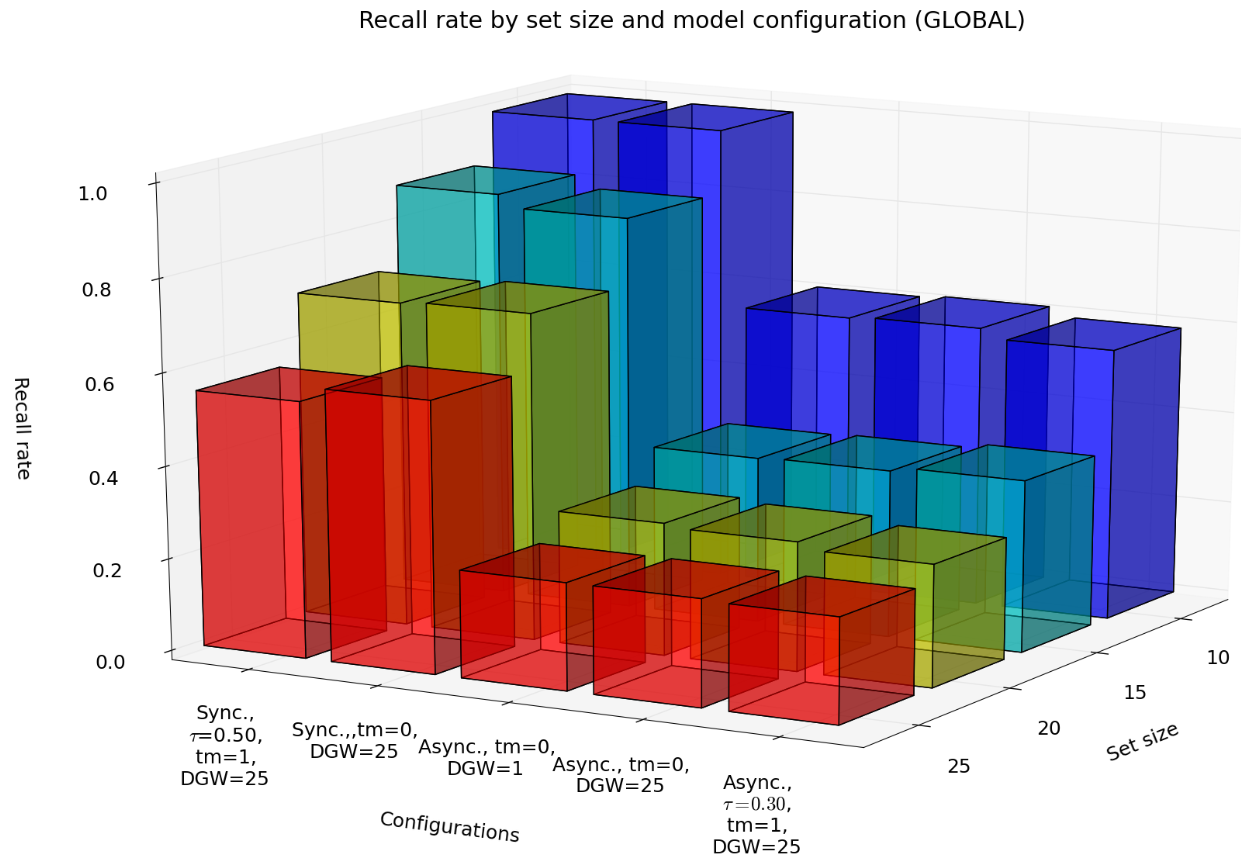
\includegraphics[width=13cm]{fig/i-iters/global-recall}
    \caption{global recall sync, async}
    \label{fig:global-recall}
\end{figure}

\begin{figure}
    \centering
    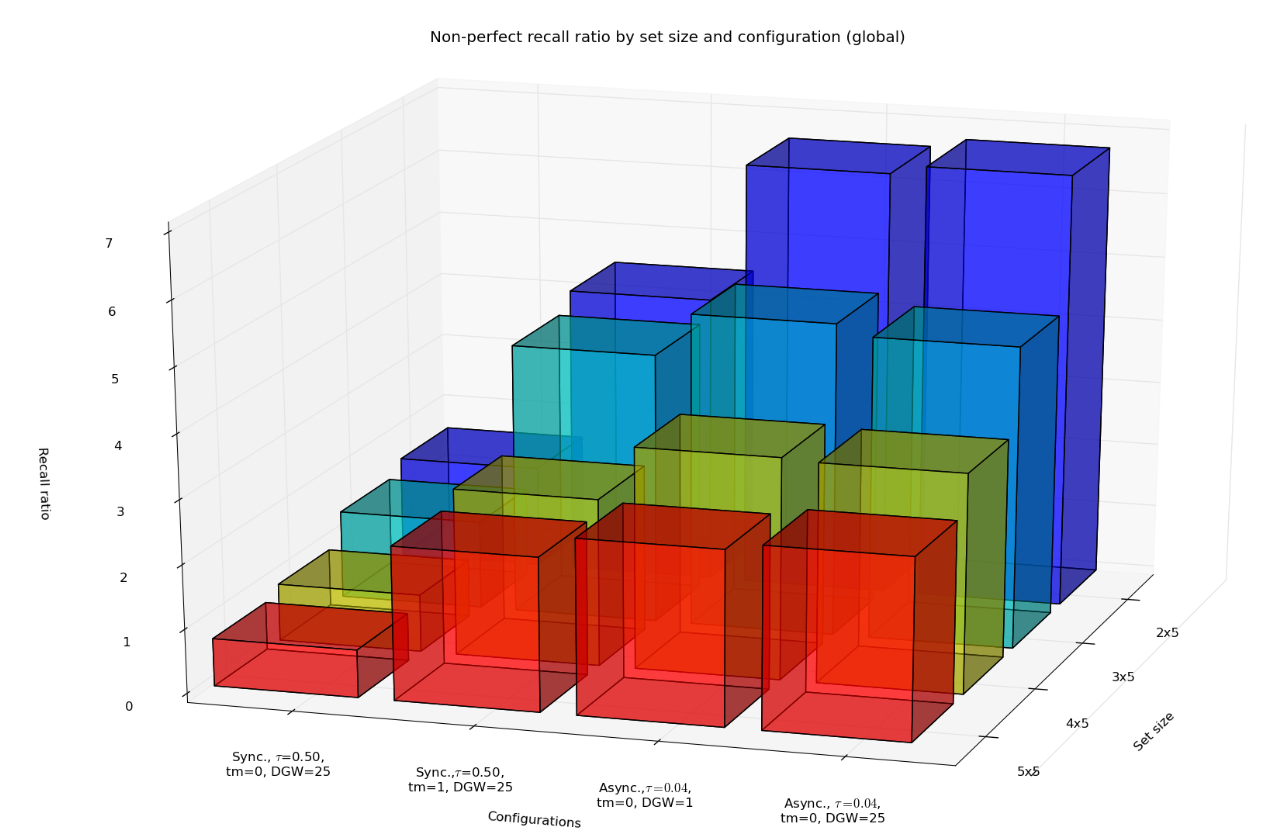
\includegraphics[width=13cm]{fig/i-iters/global-recall-spurious}
    \caption{spurious patterns for global recall sync, async}
    \label{fig:global-recall-spurious}
\end{figure}

It is worth noting that the synchronous CA3 updating scheme results in a relatively large number of spuriously recalled patterns for small set sizes. This may in indicate that the learned patterns' basins of attraction have merged, corresponding to spurious pattern(s) which may then be learned by the model. As previous empirical data, as well as the low-level demonstration has shown that the model on average successfully recalls patterns for the correct pattern input, this may point towards the issue residing within the synchronous updating schemes' recall procedure. 
Note however that once the model fails to separate two similar patterns and forms a novel spurious pattern and basin of attraction, this basin may increase the likelihood of further such spurious basins being created. This may be seen by considering that such a basin is in fact an overlap between the other basins, which is then likely to contain parts of other patterns and letters, too. In this case, the overlapping inputs will necessarily disrupt the pattern-completion of the CA3-layer, as it cannot settle into patterns that overlap too much. This phenomena has been demonstrated in work on auto-associative networks, as discussed in the background chapter, as well as in \citep{Hattori2014}, which employs a more complex HPC-model specifically to alleviate the issues of pattern separation and memory congestion in a simple Hopfield network, as is used in \citep{Hattori2010}.
Looking to the low level demonstration of the synchronous training and recall scheme, a fair stability is attained for learned pattern inputs, however, chaotic recall seems to be very unstable, only visiting learned pattern outputs for one time-step. In other words, the \textit{correct} basins of attraction have not been sufficiently consolidated for the given letters, as the output oscillates. Whether consolidation is unsuccessful due to the creation of basins of attraction for spurious pattern correlations, or only because pattern separation is unsuccessful - which necessarily renders successful learning and convergence unsuccessful, remains slightly obscure. That being said, the chaotically recalled output seems to recur only for the actual training pattern output, with spurious chaotically recalled patterns only occurring once per spurious pattern. This suggests that chaotic recall is unsuccessful largely due to unsuccessful reduction in overlap of the training patterns. One thing that could ameliorate this issue is introducing a slight neuronal turnover for every training set iteration, although less biologically realistic. If successful, it could however imply that the biological brain needs a certain randomness to its learning procedure in order to enhance its correlation extraction. This could also be more biologically realistically implemented by introducing random "noise" in between training patterns, which would introduce randomness in the eta- and zeta-equations, and thus to the chaotic neurons of the CA3-layer.
On the other hand, it may also imply that the model may be too simplified topologically speaking (which of course is the case largely speaking) with regards to attaining the desired model behaviour. More specifically, relaying the model output from CA3 to plastic connections to a CA1-layer in a more complex model, which could then relay its activity back to the EC-layer, could potentially create the recurrence needed to obtain stability in the output layer during chaotic recall. This will be further discussed in chapter 5.

% \subsubsection{50-iters training set exposure}
\begin{figure}
    \centering
    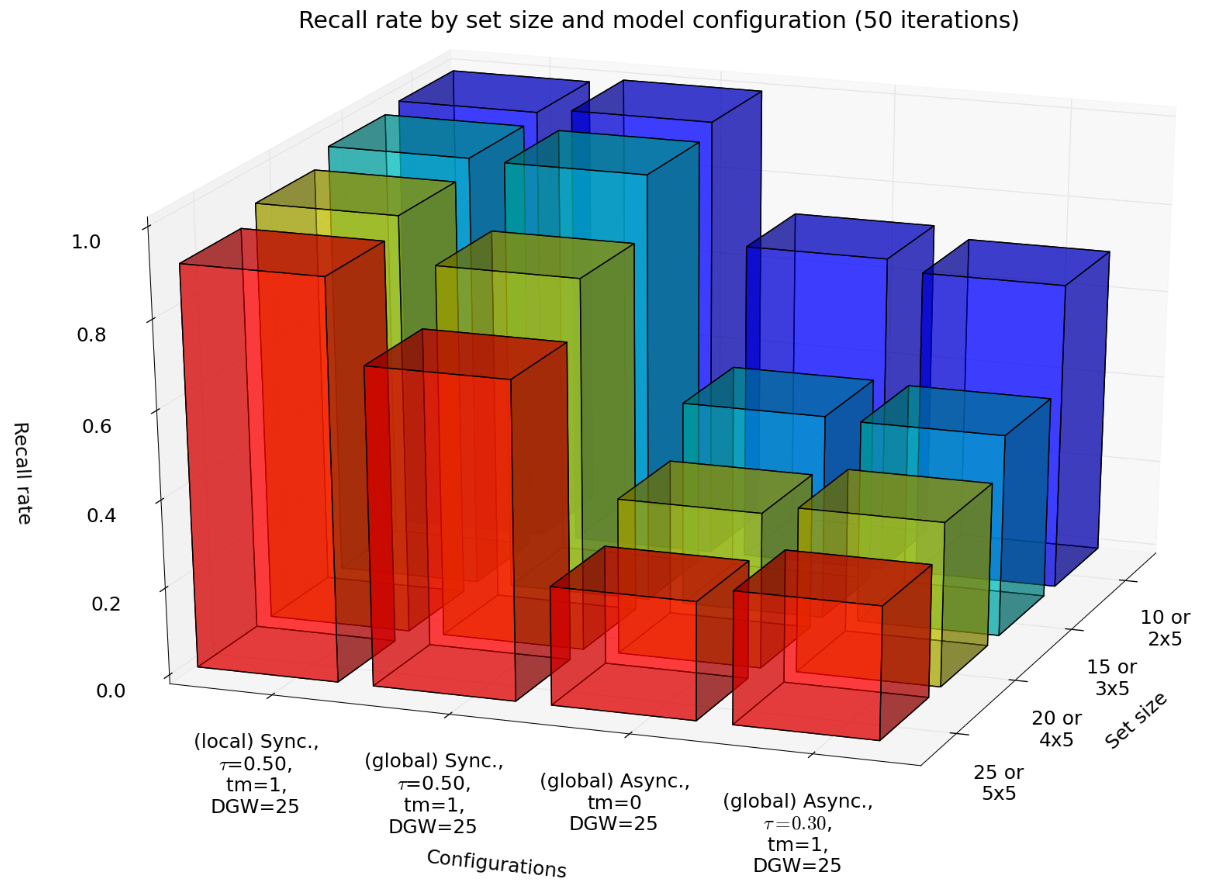
\includegraphics[width=13cm]{fig/i-iters/50-iters-recall}
    \caption{50 iters recall sync, async}
    \label{fig:50-iters-recall}
\end{figure}

\begin{figure}
    \centering
    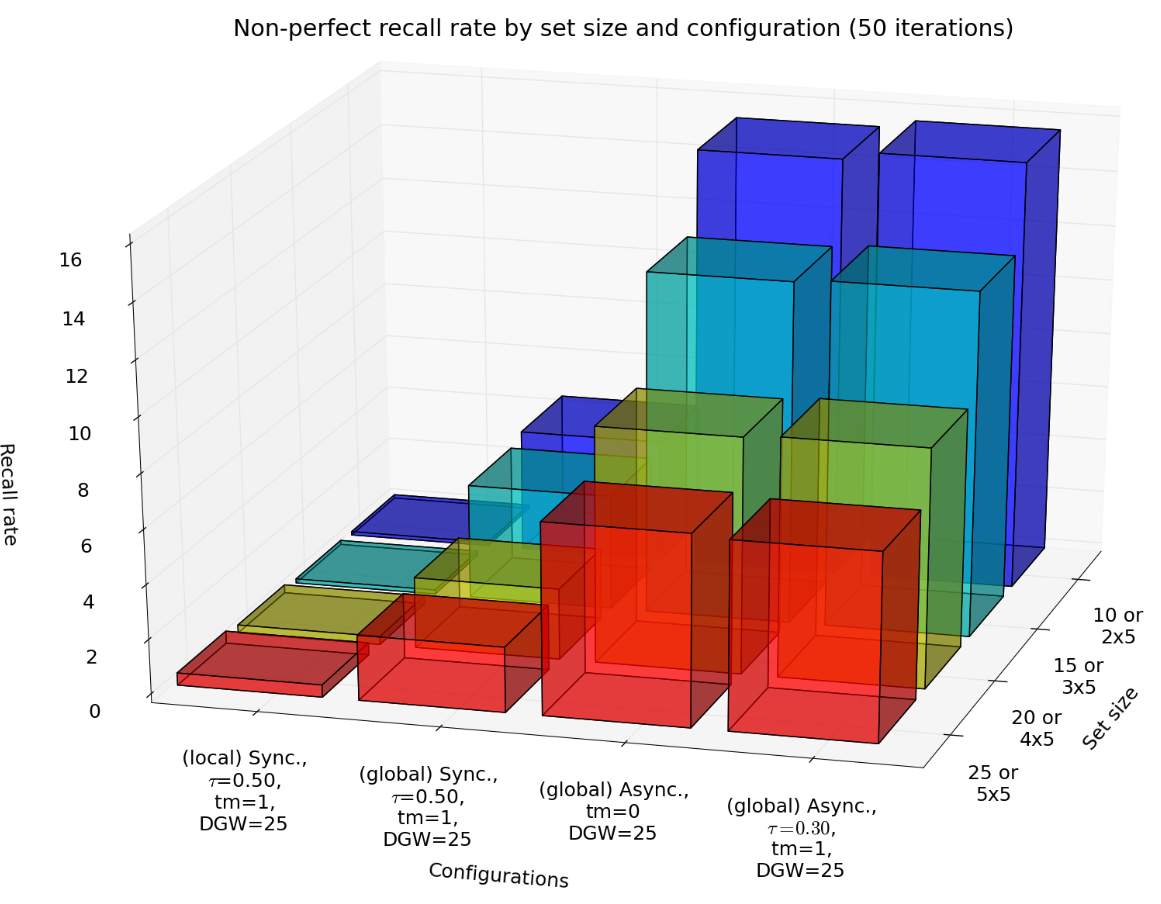
\includegraphics[width=13cm]{fig/i-iters/50-iters-recall-spurious}
    \caption{spurious patterns for 50 iters recall sync, async}
    \label{fig:50-iters-recall-spurious}
\end{figure}

When analysing the spurious recall rate of the asynchronous schemes during chaotic recall, the asynchronous schemes are in fact worse off than the synchronous scheme. Making it apparent that the potentially increased perfect recall rate for the asynchronous schemes in figures \ref{fig:local-recall} and \ref{fig:local-recall-spurious} comes at the cost of drastically increasing the number of spuriously recalled patterns. Interestingly, spurious recall is yet constrained in the synchronous updating mode. This may be due to the fact that asynchronicity simply will introduce more combinations of the previous basins of attraction, which again will lead to the output after chaotic recall being a previously unseen, distinct spuriously recalled pattern for every spurious chaotic recall iteration. However, the fact that the synchronous mode is not prone to recalling that many chaotic patterns in the global training exposure mode may shed light on previous questions asked. By considering that the perfect recall rate remains very high, but the spurious patterns extracted grows only slightly when increasing the training set size by a factor of 5, indicates that a more complete pattern-completion mechanism may be a central aspect which needs improvement in order to enhance the model performance, and possibly pattern emergent pattern separation ability.

Addressing the success observed by using neuronal turnover for every training set iteration in the synchronous CA3 updating scheme: 
This will necessarily increase the pattern separation capabilities of the model dynamically, as the model by rewiring parts of its connections thus will re-code the presented k-winners pattern to the preceding layer. However, as this is also performed for each exposure to the same pattern, it remains a bit unclear how it still enhances the separation ability. My take on this is that more randomness in re-instantiating the synapses will lead to varying the k-WTA pattern, which again will be consolidated for the successfully separated patterns dynamically, as Hebbian learning wires the neurons that are simultaneously firing, enhancing the connections that are more persistent, and thus highly correlating, more than others. Thus, re-instantiation of synaptic connections, or neuronal turnover, becomes a type of dynamic trial-and-error in pattern separation, which may be successful due to the fact that lateral inhibition is simulated by the k-WTA algorithm, which favours a certain layer-wise stability.

\subsection{Hippocampal module results summary}

Under the less stringent convergence criterion of training or recalling for 15 iterations, it became apparent that the trends for one model configuration is significantly better than the others. Namely synchronous updating of the CA3-layer neuronal activation values as well as weight updates, using turnover for every training iteration, a DG-weighting of 25, and a turnover rate of 0.50 - potentially even better for $\tau=0.30$. [THIS IS TESTED RIGHT NOW. REFACTOR?].
Anyhow - this configuration demonstrates a state-of-the-art performance for dual-network memory models in short-term memory pattern extraction and perfect recall rates. Perfect recall rates are significantly better than the models of \citep{Hattori2014, Hattori2010}. The comparative results are summarised in table \ref{table:comparison-perfect-recall-rates}.

\begin{figure}
    \centering
    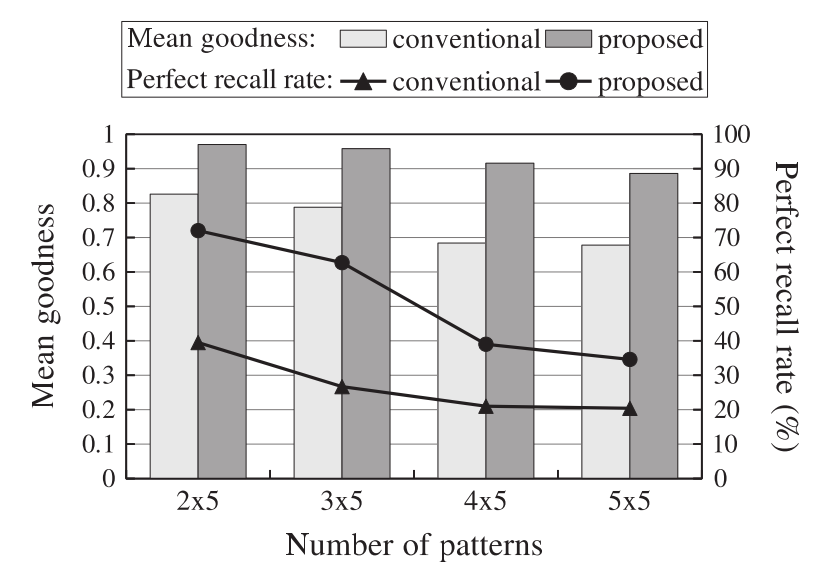
\includegraphics[width=10cm]{fig/fig6_hattori2014}
    \caption{Showing the results from \citeauthor{Hattori2014}'s \citeyear{Hattori2014} paper for hippocampal module performance for auto-associative training patterns. Displayed with permission.}
    \label{fig:fig6_hattori14}
\end{figure}

\begin{table}[]
\centering
\caption{Showing the approximate average perfect recall rate values using auto-associative training patterns for the conventional state-of-the-art model of \citep{Hattori2014}, and the novel model implemented in this thesis. See figures \ref{fig:local-recall}, \ref{fig:global-recall}, and \ref{fig:50-iters-recall} for figures illustrating the attained recall rates, and figure \ref{fig:fig6_hattori14}.}
\label{table:comparison-perfect-recall-rates}
\begin{tabular}{|c|c|c|c|c|}
\hline
\multicolumn{5}{|c|}{Perfect recall rate results}                                         \\ \hline
Pattern set size   & 2x5           & 3x5           & 4x5           & 5x5           \\ \hline
Conventional model & 0.72 & 0.63 & 0.39 & 0.35 \\ \hline
Novel model        & \textbf{1.00} & \textbf{0.98} & \textbf{0.96} & \textbf{0.9}  \\ \hline
\end{tabular}
\end{table}



% ================ Neocortical module experiments ===============
\section{Neocortical module experiments}

This section contains the experiments testing the memory consolidation to the neocortical module within the dual-network memory model. Beginning with a fairly short demonstration of convergence and interference in the outlined network with the auto-associative training set, the section is followed by a short section on pseudorehearsal, preceeded by experiments on memory consolidation from the hippocampal module. Note that 'memory' is used throughout this thesis as describing any abstract representation such as a pattern association or functional mapping inherent in the network weight configration, and thus embodied by the network itself, resulting in specific emergent network activity.

Based on the assumption that only successful extraction of patterns in the hippocampal module may provide the basis for successful information transfer to the neocortical module, the best synchronous CA3-updating mode and hippocampal configuration is selected as the model scheme for which neocortical memory consolidation is performed. Furthermore, as I wish to investigate the potential information inherent in spurious patterns, asynchronous updating scheme is also included. Consolidation using chaotically recalled patterns and hippocampal pseudopatterns is also examined in this regard, and to draw potential biological parallels.

\begin{itemize}
    \item Pseudorehearsal outline, outside scope.
    \item Demonstration of performance on original training patterns, including catastrophic interference
    \item Experiment: Using chaotically recalled patterns with random input as I, and three hippocampal pseudopattern combinations
    \item Experiment: Using the chaotically recalled output as IO for consolidation <- reduction in catastrophic forgetting through only using hippocampal patterns. Biologically plausible.
\end{itemize}

\subsection{Pseudorehearsal}

\cite{Ans1997} demonstrate that pseudorehearsal may be used to successfully reduce or eliminate catastrophic forgetting in FFBP ANNs. The mechanism which makes this possible is pseudorehearsal, as previously demonstrated by \cite{Robins1995}. Furthermore, \cite{Ans1997} demonstrate that this pseudorehearsal may be performed solely on-network. I.e. the entire previous network configuration may be transferred to another network, which may then continuously send patterns (pseudopatterns reflecting the old configuration) to the first network while the first network also learns novel patterns, thus interleaving the new patterns with old. As FFBP ANNs minimize an error-loss function, typically a distance measure from the attained output to a target output over all patterns in a training set, this results in a weight configuration which minimizes the error for both the old and the new patterns, thus attempting to maintain the new and the old information equally well, the weighting being determined by the number of patterns for each weight configuration when training using gradient-descent.
\\

While it is interesting to note that pseudorehearsal may be used to successfully interleave previously learned patterns with new, it is not my aim to demonstrate it in this thesis.
Storing patterns in a data structure that maintains the previous network configuration, and generating training patterns from this configuration in order to interleave the previous configuration with the new patterns, may also be regarded as storing the information simply in another neural network, such as demonstrated by \cite{French1997}. This remains, however, outside the scope of this thesis to demonstrate that catastrophic forgetting may be reduced to a large extent by pseudorehearsal, despite the manner in which it is performed, as this is already fairly well-documented in the literature (see chapters \ref{chpt:background} and \ref{chpt:methods} for more details on this). 
What I am addressing, is the potential information transfer capabilities inherent in the patterns produced by chaotic recall itself, as well as in the hippocampal pseudopatterns, which may supplement the chaotically recalled patterns.

\subsection{Goodness of fit}

In evaluating the performance of the neocortical module, the goodness of fit measure, $g$, is adapted from \citep{Hattori2010, Hattori2014}. It is defined as the following,

\begin{equation}
    g = \frac{1}{N} \sum_{i=1}^{N}o_it_i,
\end{equation}

where $o_i$ is the target output vector for pattern $i$, $N$ is the number of patterns in the current training set, and $t_i$ is the target output vector. Note that as the outputs are bipolar, i.e. 1 or -1, in the case of matching only 50 \% of the output, the goodness of fit will be 0.

Note that the model in being a FFBP ANN is not necessarily able to extract perfect pattern correlations, the goodness of fit measure is well suited for measuring a closeness in perfect correlation - where 1 is perfectly extracted, 0 is 50 \% - i.e. random performance, and -1 is perfectly negatively correlated.
The goodness of fit will therefore be the main measure in evaluating the consolidation quality, as well as the network performance.

\subsection{Demonstration of model performance and potential catastrophic forgetting}

Before delving into the experiments of the neocortical module, I would like to outline and demonstrate how learning of all pattern associations may be successfully attained in the feed-forward back-propagation (FFBP) network studied in this section. This may be achieved by introducing the training set as a global training set, i.e. training on every single of the say 25 patterns (in the 5x5-case) sequentially for a large number of iterations. This will lead to the successful convergence and a goodness of fit measure $g$ of above 0.99 in most cases. However, when constructing sequentially detached training sets, i.e. 5 subsets of the 25 patterns, allowing the model to train only on one subset at a time, results in catastrophic interference in the model. This brings us to the very core of the dual-network memory architecture; as everything cannot be learnt sequentially as a global training set, at least not biologically speaking, an architecture where subsets may be learnt rapidly by a short-term memory, may allow for the slow consolidation to a long-term memory such that its former memories are not disrupted.

\begin{figure}
    \centering
    
\includegraphics[width=12cm]{fig/neo-intro-demo/global_aggregate_im}
    \caption{Displaying the bipolarized recalled output for the neocortical network after it has been trained on all of the associative training patterns sequentially (as one training set) for 15 iterations. The goodness of fit of the network is $g\approx0.99$.}
    \label{fig:global_aggregate_im}
\end{figure}

\begin{figure}
    \centering
    
\includegraphics[width=12cm]{fig/neo-intro-demo/local_aggregate_im}
    \caption{Illustrating catastrophic forgetting by displaying the bipolarized recalled output for the neocortical network after it has been trained on each subsets of the associative training patterns sequentially (5x5), each for 15 iterations. The goodness of fit of the network is $g\approx0.79$.}
    \label{fig:local_aggregate_im}
\end{figure}

\begin{itemize}
    \item Global original training patterns
    \item Local training, i.e. training on each subset sequentially
\end{itemize}

\subsection{Experiment: Memory consolidation by chaotically recalled patterns}

\begin{itemize}
    \item Sync, DGW 25, tm1, $\tau=0.50$.
    \item (just to include it) Async, DGW 1 (seems irrelevant), tm0, $\tau=0.50$ (seems irrelevant)
\end{itemize}

\begin{figure}
    \centering
    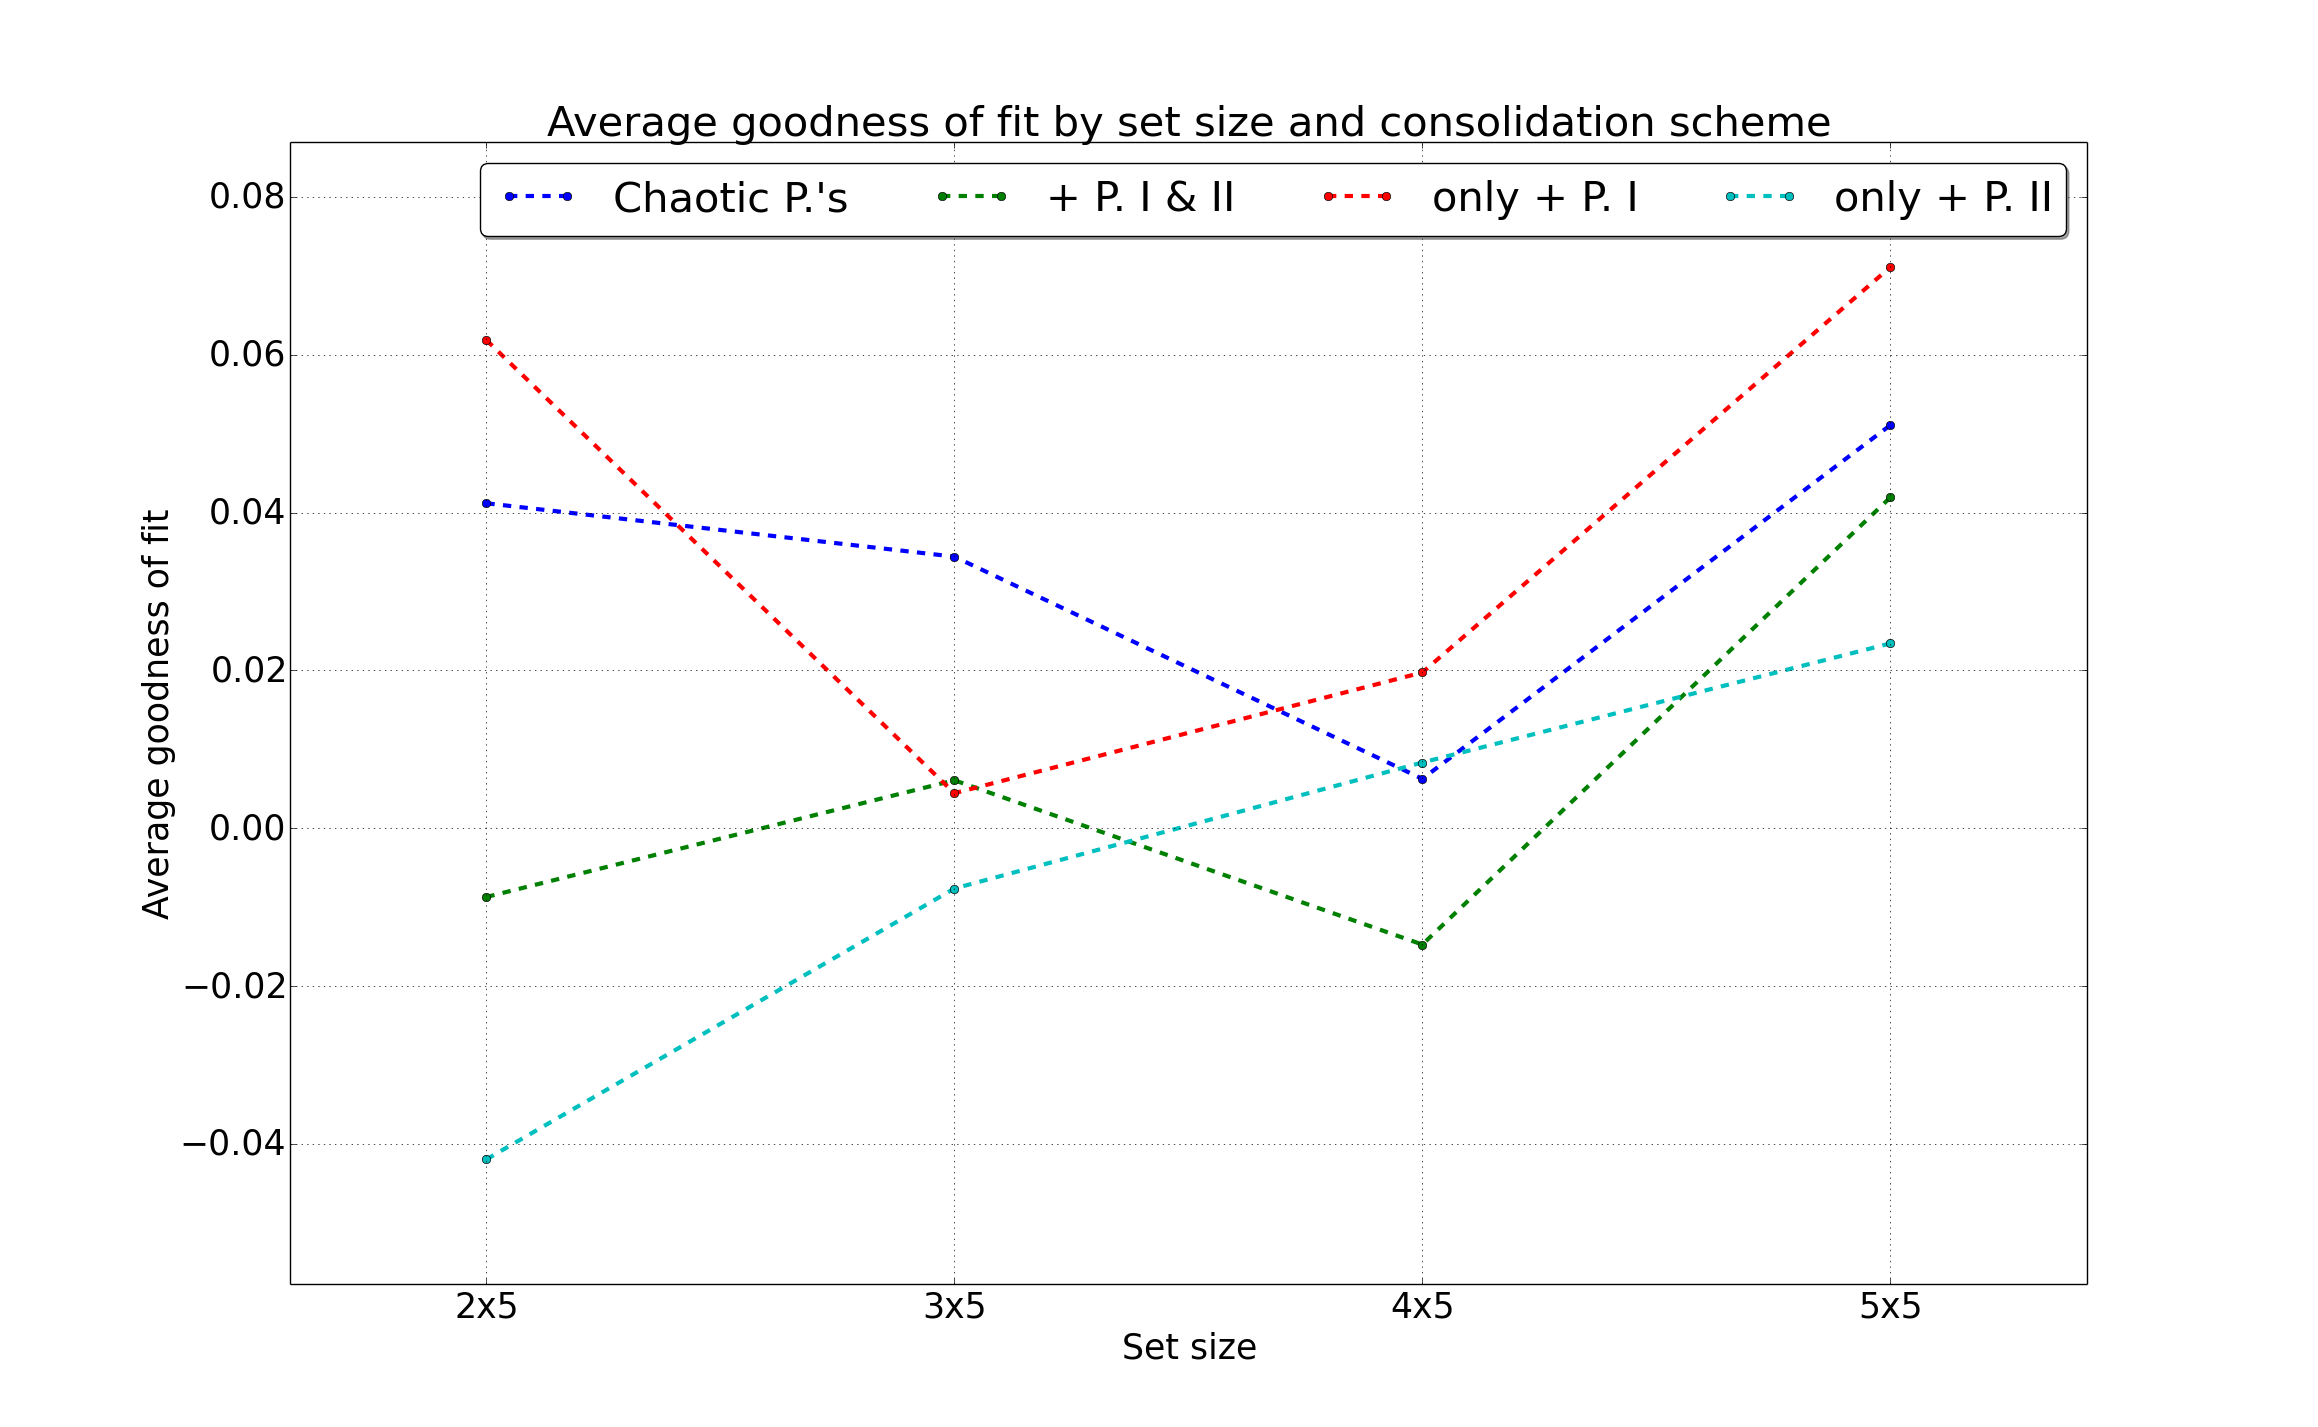
\includegraphics[width=12cm]{fig/neo-condsolidation/consolidation-schemes-sync-tm1-tr30_15_iters}
    \caption{Avg's for the two modes above. }
    \label{fig:my_label}
\end{figure}

No information seems to be transferred

\subsection{Experiment: Using chaotically recalled output as IO}

Experiment: Using the chaotically recalled output as IO for consolidation <- reduction in catastrophic forgetting through only using hippocampal patterns. Biologically plausible.

Three local schemes only:
\begin{itemize}
    \item Sync $\tau=0.30$, tm1, DGW25, 15 iters
    \item Async $\tau=0.50$, tm0, DGW25, 15 iters
    \item Sync $\tau=0.30$, tm1, DGW25, 50 iters
\end{itemize}

Low level example from one run. Some emphasis should be put on that this is novel within this thesis.

\subsection{Neocortical module results summary}

It seems that:

\begin{itemize}
    \item Solely using chaotically recalled patterns with the random input consolidates little or no information.
    \item Using the chaotically recalled patterns (output) as IO to the neocortical network reduces catastrophic interference. (Why?)
    \item Using the chaotic output as IO in the global scheme globalizes the training set, once more. This, of course, enables the FFBP ANN to extract the principal components, i.e. minimize the error-loss function in the weight-space spanning across all of the chaotic pattern outputs. This results in a performance (goodness of fit) near the case of simply iterating over the entire original training set, but results in lesser performance.
\end{itemize}

In other words, the mechanism of using the chaotically recalled pattern ouputs as IO to the neocortical network ameliorates catastrophic interference, but only in the local training scheme. This is interesting.

\subsubsection{Notes}

Because convergence, as well extraction, was poorer under the first convergence criterion, these schemes are not used to analyse chaotic pattern consolidation.
Intuitively speaking, as patterns are extracted by chaotic recall, there is obviously some information contained in the output, as the output is that of a previously learnt pattern.

this may be regarded as the process occurring under the inclusion of CA1, which may then relay the output back to the EC. furthermore, this output may then be slightly recoded, and thus the IO-pattern also more SEPARATED in the weight space. this would then in fact reduce interference and increase the quality of learning and performance according to the goodness of fit in the neocortical module.


% ================ Hetero-associative training patterns ===============
\section{Hetero-associative training patterns}






% ========================== RESULTS ============================
\section*{Result notes}

right now: attempt to even out the consolidation patterns in weight space. does not seem to have a direct impact.

Although possibly unrealistic, spanning outputs for chaotically recalled patterns and creating a global training set results in a goodness of fit near 1, which is nearly the same performance as for the clean, undistorted, globalised training set - i.e. the best possible performance.
When training on the subsets sequentially, the performance drops to the 0.7-0.8 interval. HOWEVER, when training on the subsets constructed by spanning over the chaotically recalled OUTPUT, performance rises significantly; > 0.8.
This may suggest that information separating the patterns in weight space is contained within the spuriously generated patterns. Furthermore, when inspecting the experiments in which the best consolidation quality was achieved using local training of the neocortical module, large numbers of spurious patterns were present. In fact, the empirical data, as well as figure [not yet created], strongly suggests that the spurious patterns are crucial to consolidating the patterns to the neocortical network. Furthermore, they seem to be enabling interleaving of old memories with new implicitly. I hypothesise that this is either by stimulating the long-term memory network in such a way that the weight configuration is less disrupted, or because the strongest pattern-correlation information is contained within these spurious patterns, thus increasing the goodness of fit measure. Addressing the first hypothesis: It may be suggested that this is a viable and fairly biologically realistic mechanism for interleaving patterns, which of course will be in synthesis with further mechanisms, by considering that the output may in fact be relayed back by the CA1-layer, and thus the EC and CA1 activity may be relayed to a long-term memory network, where the chaotically recalled pattern may span a network, stimulating it for consolidation. By considering that FFBP ANNs may be regarded to in fact attain fairly biologically realistic properties on the network level, in contrast to prior historical belief within the field, this view is not implausible.
Addressing the latter, less complex hypothesis; it is likely that the spurious patterns reflect to some extent the current and former network configuration, as the activity after a constant, continuous flow of recall has occurred. Therefore, I regard the latter as the most likely explanation. Note, however, that this does not disregard the possible implications for how biological consolidation mechanisms might work.


% ========= for all ==========

some patterns may be recalled after the next training set has been learned. i allowed this to put the pattern in the set of chaotically recalled patterns, because it reflects something which is fairly stable in the hippocampal module.
\\

Async. seems to be by far the most accurate in terms of perfect recall when it converges. Sync. with turnover for every learnt set has the highest convergence rate - non-changing for different set sizes, but the worst perfect recall rate.

It would be very interesting to see how using the 'spurious' patterns along with the actual matching patterns would consolidate to the neocortical network, comparing this to the performance attained by using the formerly outlined pseudopattern generation. In the event of having a similar effect from pattern consolidation using spurious patterns, this may point in the direct
ion of spontaneously generated 'spurious' patterns in fact possibly acting as pseudopatterns, thus outlining a process for pseudopattern generation in the brain. (Where the stability during recall could determine the consolidation strength. For complete convergence during training using async, mode 0, about 7 iterations were required for convergence - which is thought to be (?) the number of required iterations for successful neocortical memory consolidation. This could be a spurious correlation - however, the number is equal during convergence for set size 2. If the same number of iteration can be required for a successful configuration for set size 3, this would suggest that the number is not spurious.)
\\

Along with the spurious patterns, if considering the sum of distinct perfectly recalled patterns and spurious patterns as containing information about the number of patterns, the asynchronous scheme seems to contain the most information, only falling off at set size 5. This is most likely due to the convergence being 0 \% , which it actually is at set size 4, too. Increasing the number of iterations may remedy this - however, a further calibration is most likely more relevant.
\\

The recall rate is much better for the same convergence rate in the asynchronous scheme, which points towards this being the preferable scheme. Furthermore, because turnover for every set iteration remains biologically implausible, a more plausible, yet still unrealistic model should be chosen. I.e. Async., turnover for every new set.

STD only log() in async. -> points to more stable/realistic mechanism?
\\

Gradual exposure through the constant output of the HPC during recall and learning? If this may consolidate something to the PFC, it would be really interesting.
\\

In order to target the black-box analysis that analyzing an ANN can be - particularly for the case of biologically realistic networks using chaotic neurons - I employed a type of logging, from which data is parsed, and sorted by a parser that I wrote. This data includes the number of spurious patterns extracted, where spurious is defined as not perfectly overlapping any of the provided training patterns. Furthermore, it includes the number of iterations before convergence, where 50 iterations is considered as failure to converge. It also includes the weighting selected for the connections from the DG, the neuronal turnover rate that was employed, and lastly the number of extracted patterns, along with the perfect recall rate for the current experiment.
\\

appears to be a significant correlation between the convergence rate and the perfect recall rate. this probably correlates with most positive emergent attributes that we wish to attain in the HPC network


% ========================== section ============================
Experiment design
Results
Comparisons

\section*{Notes}

Enforce sparsity through weight updates corresponding only to the winners of kWTA - didn't work.

\textbf{100 \% connection ratio EC-CA3:}

Fairly rapid convergence for three patterns in HPC-module for turnover between every training set iteration. 
Not necessarily successful recall of all patterns. Does this have something to do with the synchronized CA3-layer during recall? Separation possible during recall when the desired pattern(s) are presented to the network - however, not all may be recalled.

-> New random pattern each time stability was reached resulted in better recall.

Is this also the case for heavier weighting of the DG-CA3 path during learning?

Spurious pattern reduction/correlation with occurrence when using turnover?

Convergence when turnover is removed between set iterations?

Heavier weighting DG. Based on paper \citep{Norman2003}. Empirical results. Chpt. 4. Figures. Nice.

\section*{Model calibration}

Experiments designed for model calibration

Dimensions analyzed outlined above.

First: STM-network extraction rate (at first, empirically observed to be same as solely auto-associative Hopfield network).


\textbf{Notes}

experiments suite - two as outlined by \citep{Hattori2014}, originally retrieved from ... as outlined above
enabling several trials automatically.

Turnover between every training set iteration (?). Needs to include empirical data on decision making. Move to preliminary experimentation in chpt. 4?
\\

It would be interesting to see HPC expanded to include neo. nets activity fed back into the hpc net. in order to induce activity. Perhaps this may cycle through previous patterns. Expanding the model towards Wakagi (08), and using a kind of reverberation could be a focal point in future work.

async. seems in one way more robust, i.e. less affected by the changing parameter settings. is this because it is incapable of convergence in all config.s?? (dgw and taus no major impact on prrs)

Possibly subsets of neurons doing updates synchronously, so subset asynchronicity. Might be that async. is unsuccessful in convergence due to separation.


\cleardoublepage
